\documentclass[12pt]{book}              
%\parindent0pt  \parskip10pt             % make block paragraphs
%\raggedright                            % do not right justify

\usepackage[margin=2cm]{geometry}
\usepackage{enumitem}
%\usepackage{url}
%\usepackage{siunitx}
\usepackage{listings}
\usepackage{graphicx} 
\usepackage{booktabs} % for much better looking tables
\usepackage{array} % for better arrays (eg matrices) in maths
\usepackage{verbatim} % adds environment for commenting out blocks of text & for
\usepackage{subcaption} % make it possible to include more than one captioned fi
\usepackage{float}
\usepackage[hyperfootnotes=false]{hyperref}
%\floatstyle{boxed} 
\restylefloat{figure}
\usepackage{tabularx}

\lstset{
%  framexleftmargin=10mm, 
%  tabsize=2,
%  language=c, 
  frame=single,
  numbers=none,
  keepspaces,
%  basicstyle=\footnotesize,
  basicstyle=\scriptsize\ttfamily,
}


%%%% insert figures %%%%
% Args: 1=page in pdf file with figure (1, 2, etc)
% 2=scale factor (1: no scale, 0.5: reduced to 50%, 2:double, etc)
% 3=caption
% NOTE: defines label f-page_nr for each figure
\newcommand{\inspdf}[3]{
\begin{figure}[tb]
\begin{center}
\includegraphics[page=#1, scale=#2]{figs-manual/figs.pdf}
\end{center}
        \caption{#3}\label{f-#1}
\end{figure}
}
\pdfpagebox5

\usepackage{tcolorbox}
\usepackage{xcolor}

\usepackage[
    type={CC},
    modifier={by-sa},
    version={4.0},
]{doclicense}


\title{Computer Networks - Laboratory manual}    % Supply information
\author{Robert Benkoczi, University of Lethbridge}    %   for the title page.
\date{\today\\ version 3.3.3}  %   Use current date. 

%%%%%% macros %%%%%%5
\newcommand{\kathara}{Kathar\'a}

%%% inserting figures 
%%% arg 1: figure file (no directory)
%%% arg 2: scale factor
%%% arg 3: caption
%%% labels are #1.fig
\newcommand{\insfig}[3]{
\begin{figure}[tb]
\begin{center}
\includegraphics[scale=#2]{figs-manual/#1}
\caption{#3\label{#1.fig}}
\end{center}
\end{figure}
}

\setcounter{chapter}{-1}

%\newenvironment{console}
%               {\begin{scriptsize} \begin{verbatim}}{\end{verbatim}  \end{scriptsize}}

%%%%%%%%%%%%%%%%%%%%%%%%

%\renewcommand{\chaptername}{Activity}

% Note that book class by default is formatted to be printed back-to-back.
\begin{document}                        % End of preamble, start of text.
\frontmatter                            % only in book class (roman page #s)
\maketitle    
\doclicenseThis                      
\tableofcontents                        % Print table of contents

\mainmatter % arabic page nrs

\chapter{Introduction}

This manual documents the lab work for course CPSC 3780 Data Communications and Networking at the University of Lethbridge. There are two types of lab activities described in this manual. The first, introduces network programming techniques. The second, teaches basic network management tools that will help with understanding several basic network protocols.

Network programming follows a slightly different model from the typical sequential programming paradigm so familiar to C++ programmers, and thus the lab sessions in Part \ref{cpp.part} introduce some system programming tasks such as running and synchronizing threads, working with binary structured data, and sockets.
The lab sessions in Part \ref{kathara.part} introduce the students to some of the network management tools currently used in practice. It provide hands-on experience with some basic tasks in network management, using a networking emulation package called \kathara.


%%%%%%%%%%%%%%%%%%%%%%%%%%%%%%%%%%%%%%%%
\part{Network programming}\label{cpp.part}
%%%%%%%%%%%%%%%%%%%%%%%%%%%%%%%%%%%%%%%%%%%5

%%%
\chapter{Lab N1: Network programming}

In this part of the lab, students will explore the programming libraries that will help them complete the project for the class. Network programming requires processing asynchronous events and this can be handled with multiple threads of execution. Threads can be avoided with advanced operating system calls such as \emph{select}, but I feel threads can be useful in other situations as well, so there is no harm in learning to program them. We start with basic multi-threaded programming and thread synchronization approaches. 

\section{Objectives}

Students will write a C++ program that starts several threads. The program will end when all threads end.

\begin{enumerate}[label=Objective \arabic*]
\item\label{thread.start} Using the C++ STL, students will write code that starts threads of execution.
% \item\label{thread.sleep} Students will write code that can wait (sleep) for a given period of time.
\item\label{mutex} Students will use a mutex object to exclude concurrent execution of portions of the code in a multi-threaded environment.
\item\label{lock.guard} Students will control the mutex through a \lstinline$lock_guard$ object that guarantees a safe lock/unlock mechanism.
\end{enumerate}


\section{Summary of routines}

\begin{tabularx}{\textwidth}{r  X}
  C++ Class or routine & Description \\ \midrule
  \lstinline$std::thread$ & spawns a new thread when a thread object is constructed  \\
  %  \lstinline$std::this_thread::sleep_for$ & puts currently running thread to sleep
  \lstinline$std::mutex$ & when locked, any other attempts to lock the mutex by other processes will block the processes \\
  \lstinline$std::lock_guard$ & an object that manages mutexes
\end{tabularx}

\section{Lab activities: warm-up}

\begin{enumerate}[label=Activity \arabic*:]
  
\item Consider the following output function:

  \begin{lstlisting}[language=C++]
    void print(int n, char c) {
      for (int i = 0; i < n; i++) {
        std::cout << c << std::flush << ' ' << std::flush;
      }
    }
  \end{lstlisting}

  Examine the code and explain what this function does.

\item Create a working directory and a source file called \emph{sequential.cc} inside. Include the \emph{print} function and define \emph{main} to call \emph{print} twice. An example is shown below. Compile and execute your program.

  \begin{lstlisting}[language=c]
    int main() {
      print(100, 'a');
      print(100, 'b');
      return 0;
    }
  \end{lstlisting}

 The output modifier \lstinline$std::flush$ forces the output operator to immediately produce the output. Normally, the output produced by the output stream operator is buffered and there is no guaranteed time when the output is actually sent to the console.


\end{enumerate}


%% \subsection{Lab activities: \ref{thread.sleep}}

%%   \begin{enumerate}[resume*]
%%   \item We can modify function print to slow it down a little. This will help us appreciate the behaviour of the program once we start using threads. In the for loop of print, instruct the program to sleep for 50 ms after each output character.

%%     \begin{lstlisting}[language=c]
%%       void print(int n, char c) {
%%         for (int i = 0; i < n; i++) {
%%           std::cout << c << ' ' << std::flush;
%%           std::this_thread::sleep_for(std::chrono::milliseconds(50));
%%         }
%%       }
%%     \end{lstlisting}

%%   \item Examine the documentation for the helper class \verb$milliseconds$ and for the function \verb$sleep_for$. Use \url{cppreference.com}. Are there any other helper classes to represent duration?

%%   \item Compile and execute the program. Choose other values for the wait time and re-run.
%%   \end{enumerate}


  \subsection{Lab activities: \ref{thread.start}}

  \begin{enumerate}[resume*]
  \item Copy your code from file \emph{sequential.cc}  into a file named \emph{parallel.cc}. Modify the main function to change the first call to print into spawning a thread that executes the print function. Make sure to \lstinline$#include <thread>$. Compile and execute.

    \begin{lstlisting}[language=c]
      int main() {
        std::thread t1(print, 100, 'a');
        print(100, 'b');

        t1.join();
        
        return 0;
      }
    \end{lstlisting}

    Calling \verb$join$ on a thread blocks the calling process until the thread finishes execution.

    \item Change function \verb$main$ so that both print function calls are executed by a parallel thread each.
  \end{enumerate}


  \subsection{Lab activities: \ref{mutex}}

  \begin{enumerate}[resume*]
  \item When we run the \emph{parallel.cc} example, we may notice that the output produced is not always nicely arranged. The console output from one thread may occur between the output of the character and the space of the other thread. Suppose that we consider one iteration of the for loop in \emph{print} a \emph{critical section} and we want to ensure that no other thread is outputting until the iteration ends.

    We can use a mutex (MUTual EXclusion) to limit the parallel execution of portions of the code. See \url{https://riptutorial.com/cplusplus/example/26751/mutexes---thread-safety} for more details.

    Copy the code from file \emph{parallel.cc} into file \emph{parallel-mutex.cc}. Define a mutex object as a global variable. Lock the mutex at the start of the loop iteration, and unlock the mutex at the end.

    \begin{lstlisting}[language=c]
      std::mutex print_mutex;
     
      void print(int n, char c) {
        for (int i = 0; i < n; i++) {
            print_mutex.lock(); 
            std::cout << c << std::flush << ' ' << std::flush;
            print_mutex.unlock();
        }
      }
    \end{lstlisting}

  \item Compile and run. What do you notice?

  \item Modify the code to change the declaration of \lstinline$print_mutex$ from a global variable to a variable local to function \emph{print}. Compile and run. What do you notice

    \item Modify the code back with a globally declared mutex. Then, comment out the call to unlock the mutex. Compile and run. What do you notice. Explain.
  \end{enumerate}


  \subsection{Lab activities: \ref{lock.guard}}

  \begin{enumerate}[resume*]
  \item The lock/unlock mechanism on a mutex is prone to errors. Forgetting to unlock a mutex can lead to a deadlock. In C++, we can manage a mutex using a \lstinline$lock_guard$ object. A lock guard locks a mutex when the lock guard is constructed and unlocks the mutex when the lock guard is destructed.

    Copy the code from file \emph{parallel-mutex.cc} into file \emph{parallel-lock-guard.cc}. Modify the \verb$print$ function as follows.

    \begin{lstlisting}[language=c]
      void print(int n, char c) {
        for (int i = 0; i < n; i++) {
          // this block statement is executed as an atomic operation;
          {
            std::lock_guard<std::mutex> lock(print_mutex); // construction locks the mutex
            std::cout << c << std::flush << ' ' << std::flush;
          }    // destruction unlocks the mutex 
        }
      }
    \end{lstlisting}

    Compile and execute.
  \end{enumerate}

  \subsection{Conclusion}

  Use the thread class to start parallel threads. Declare a mutex and create a \verb$lock_guard$ object to manage the mutex and to avoid concurrent execution of certain portions of your code.


  \section{Exercises}

  \begin{enumerate}[label=\arabic*.]
  \item Write code that spawns 30 parallel threads. Each thread is executing the \verb$print$ function illustrated in the lab activities. Please end the main program when all threads spawned are finished. Submit two source files, one in which a lock guard is used to protect each iteration of the for loop in print, and one where no mutex or lock guard is used. Submit also screen shots with the execution of the two programs. Hint: store thread objects in an array.


  \item Write a program that spawns 4 parallel threads. Two of the threads use one queue data structure (the same queue) to insert randomly generated integers. The other two, extract the integers from the queue. Protect the Queue with a mutex managed by a lock guard. The inserting threads should generate 100 integers each. After generating the integers, the generating threads should end. Design a mechanism by which the extracting threads end their execution when no more data is inserted by the generating threads because they terminated. Output appropriate messages to identify each operation with the queue and reveal which thread executes it. 
  \end{enumerate}


%%%%%%%%%%%%%%%%%
\chapter{Lab N2: timers}

In this lab, students will use STL classes to implement the timer functionality needed when programming the typical action-confirmation network protocol behaviour. In this scenario, a process performs an action such as sending a data packet to a peer process, and then it waits to receive a confirmation from the peer process. The confirmation may or may not arrive. If the confirmation arrives, the sending process should resume execution right away. If the confirmation does not arrive, the sending process should resume execution after a maximum wait time (the timer value). The sending process must be able to distinguish the two cases - confirmation received or timer expired. We can implement this behaviour with a \emph{condition variable} object from the STL.

In the second part of the lab, students will design, implement, and test a class whose responsibilities are to manipulate the fields of a packet header.

\section{Objectives}

\begin{enumerate}[label=Objective \arabic*:]
\item\label{unu.l2} Students will explore the signaling features of a condition variable object. Students will also compile and build simple programs using condition variables. 
\item\label{doi.l2} Students will implement an expiration timer using condition variables.
\item\label{trei.l2} Students will design, implement, and test a class responsible for writing and reading the various fields of the header for the course transport protocol. The course transport protocol is the course project for CPSC 3780.
\item\label{patru.l2} Students will use the \emph{Google test} framework (refer to CPSC 2720) to test their class.

\end{enumerate}

\subsection{Summary of classes}

\begin{tabularx}{\textwidth}{r  X}
  Classes & Description \\ \midrule
  \lstinline$std::condition_variable$ & class with various process signaling responsibilities; see \url{https://cplusplus.com/reference/condition_variable/condition_variable/} \\
  \lstinline$std::mutex$ & blocks threads  when trying to lock a mutex more than once\\
  \lstinline$std::unique_lock$ & manages a mutex and implements a more complex locking and unlocking protocol \\
  \lstinline$wait_for$ & member function of condition variable; uses a \lstinline$unique_lock$ to wait for a given period of time or until notified through the condition variable, whichever occurs first
\end{tabularx}


\subsection{Lab activities: \ref{unu.l2}}

A condition variable can be used by threads to signal each other. We can explore these features next.

\begin{enumerate}[label=Activity \arabic*:]

\item\label{pa2.unu} A condition variable can be constructed using the default constructor. Since condition variables are used for signaling, important  member functions are the \emph{notify} functions. 

  Write a program that constructs a condition variable and then notifies the condition variable.

  \lstinputlisting[title=2-notify.cc]{src/2-timers/2-notify.cc}

\item Compile and execute the program:

  \begin{lstlisting}
$ g++ -o 2-notify -lpthread 2-notify.cc 
$ ./2-notify 
Before notify
After notify
  \end{lstlisting}

  What do you notice? A condition variable can only be constructed using the default constructor. We can then invoke the notify functions, but nothing interesting happens because there is no other thread using the condition variable.

\item Modify the code from \ref{pa2.unu} to create two threads that use the same condition variable.

  \lstinputlisting[title=2-threads.cc]{src/2-timers/2-threads.cc}

  Compile and run the program several times. What do you notice? Nothing interesting, the threads that call \emph{notify} repeatedly on the condition variable don't seem to be affected by the condition variable.

\item In order for some interaction to happen between threads, one of the threads should \emph{wait} and block on the condition variable. The wait functions require a lock on a mutex to be able to wait.

  Write a program with two threads. One thread, the sleeper, waits on the condition variable. The other notifies the condition variable after a delay of 1 sec. Compile, run, and check that the sleeper thread wakes up.

  \lstinputlisting[title=2-sleeper.cc]{src/2-timers/2-sleeper.cc}
\end{enumerate}

\subsection{Lab activities: \ref{doi.l2}}\label{wakesleep.se}


\begin{enumerate}[resume*]  
\item Extend the program above so that the sleeper thread uses the \lstinline$wait_for$ function on the condition variable. Perform the following changes to the source code:
  \begin{itemize}[label=--]
  \item Replace the wait function by \lstinline$wait_for$ in the sleeper thread. The sleeper should wait for 1 sec.
    
  \item Test the return value from the wait function in the sleeper. If the return value equals \lstinline$std::cv_status::timeout$, then the timer expired before the sleeper was notified, otherwise the sleeper was notified and resumed execution. Out a message from the sleeper thread to identify if the sleeper thread was notifies by the waker or if the timer for the wait expired.

  \item In the waker, change the initial wait time from 1 sec to a random value between 0 and 2 sec, so the waker notifies the sleeper after waiting for a randomly chosen period of time. Use the \lstinline$std::rand()$ function to generate a random value between 0 and 2000 milli sec. Use \lstinline$std::srand(std::time(NULL));$ to seed the random number generator.
  \end{itemize}

  Compile the program and run it repeatedly. What do you notice? You should see that in approximately half of the runs, the sleeper timer expires. 
  
\end{enumerate}

\section{Exercises}

\begin{enumerate}
\item Starting from the waker/sleeper source code developed in Section \ref{wakesleep.se}, extend its functions so that the following features are available:
  \begin{enumerate}[label=\alph*)]
  \item There are two sleeper threads.
  \item The waker can randomly choose to wake one of the sleeper threads or the other. The other thread's waiting period expires.
  \item Output messages should clarify which operations are carried out by threads and by which threads. In particular, you should assign an ID to each of the sleeper threads, for example, by passing the ID as an argument to its function.
    \item Explain your approach in a short PDF report: are you using different condition variables? Are you using the same condition variable? Justify your choices. 
  \end{enumerate}
\end{enumerate}




%%%%%%%%%%%%%%%%%
\chapter{Lab N3: packet headers}

In this lab, the students will start to develop code for setting and extracting information from binary packet headers. 

\section{Objectives}

\begin{enumerate}[label=Objective \arabic*]
  \item\label{pl3.maps} Students will read and create bit header maps for various headers. 
\item\label{pl3.bit} Students will use shift and bit-wise operations to set and get bit fields that are smaller than 8 bits.
\item\label{pl3.byte} Students will use shift, bit-wise, and array access operations to manipulate numerical fields that are multiples of 8 bits, stored in big-endian or network byte order.
\item\label{pl3.head} Students will modify a C++ class that manipulates header fields. Students will use Google tests to test this header management class.
\end{enumerate}

\subsection{Resources}

\begin{itemize}[label=--]
\item Bit-wise and shift operators in C++: \url{https://www.geeksforgeeks.org/bitwise-operators-in-c-cpp/}
\end{itemize}


\section{Lab activities}

\subsection{\ref{pl3.maps}}

You can work on the following activities in groups, if you wish.

\begin{enumerate}[label=Activity \arabic*:]
\item Most networking layers add information to the packets they handle. This information is usually added at the beginning of a packet and is stored in binary form, to minimize the length of the packet.

  The structure of the information is represented by a \emph{header map}, a representation that lists the location of various numerical values in a table like format. Columns in this format may identify bits fields. For example, an array of 3 byte values can be shown as follows.

\begin{verbatim}
  0        7
 +----------+
 |  1st val |
 +----------+
 |  2nd val |
 +----------+
 |  3rd val |
 +----------+
\end{verbatim}

An array of two 16 bit numerical values can be shown as follows.
\begin{verbatim}
  0               15
 +-----------------+
 |  1st 16 bit val |
 +-----------------+
 |  2nd 16 bit val |
 +-----------------+
\end{verbatim}

A header containing fields of different sizes: the field \emph{Val} is a 2 bit value stored as the most two significant bits of the first byte in the header; the \emph{payload} is a 16 bit value stored starting with the 16-th bit in the structure.
\begin{verbatim}
 0   1 2   7 8  15 16     31
+=====+=====+=====+=========+
| Val | unu | unu | payload |
|     | sed | sed | length  |
+=====+=====+=====+=========+ 
\end{verbatim}

On a sheet of paper, sketch an updated header map that consists of the Val and payload length fields above + two other 16 bit values, labeled A and B.


\item In the diagrams, small bit indices correspond to the most significant bits in a byte. Similarly, multi-byte values are stored in network order (big endian): most significant byte is stored first (at the lowest numbered byte). For example, if we identify the payload length by its most significant and least significant byte, payload length = MSB LSB, then this will be stored as follows.
\begin{verbatim}
 0   1 2   7 8  15 16  23 24   31
+=====+=====+=====+=============+
| Val | unu | unu | MSB  | LSB  |
|     | sed | sed |      |      |
+=====+=====+=====+=============+ 
\end{verbatim}

Assuming that the unused bits are zero, write the value of the header above in hexadecimal format if Val is 3 and payload length is 0x214a.

\item Suppose we change the header and denote bits 2-7 by X.
\begin{verbatim}
 0   1 2   7 8  15 16  23 24   31
+=====+=====+=====+=============+
| Val |  X  | unu | MSB  | LSB  |
|     |     | sed |      |      |
+=====+=====+=====+=============+ 
\end{verbatim}

Provide the value of the header if Val is 2 (in decimal), X is 51 (in decimal), and payload length is 0x31af (in hexadecimal).
\end{enumerate}


\subsection{\ref{pl3.bit}}

\begin{enumerate}[resume*]
\item Review the meaning of bitwise operations in C++. Note that all bitwise operations involve byte values. For example, if $b_1 = 1000.0100$ and $b_2 = 0100.1100$ then the bitwise OR between $b_1$ and $b_2$ is $1100.1100$.

  What is the bitwise AND between $b_1$ and $b_2$?

  What is the bitwise OR between the byte values 0xA and 0x5? What is the bitwise AND between these values? What are the bitwise OR and then the bitwise AND between 0xA and 0x6? Consult online resources to answer these questions.

\item Write a small C++ program that reads two positive integers in the range 0-255 from the input and then it outputs the result of the bitwise AND between these values in hexadecimal. Consult the STL documentation detailing the output stream functions and manipulators. Test with the values 0xA (10) and 0x6 (6).
  
\item Consider the first byte in the header above. Suppose we want to assign  field Val the value 2 while keeping the value of X unmodified.

\begin{verbatim}
 0   1 2   7 
+=====+=====+
| Val |  X  |
|  1  |     |
+=====+=====+
\end{verbatim}

  One way to do this is to create two byte values that we then bitwise OR together, as shown below.

\begin{verbatim}
 0   1 2   7 
+=====+=====+
| Val |  X  |
| 00  |     |
+=====+=====+
  bitwise OR
 0   1 2   7 
+=====+=====+
| Val | 000 |
|  2  |     |
+=====+=====+
\end{verbatim}

Write a small C++ program that reads one byte value from the input (a positive integer in the range 0-255) and clears the two most significant bits corresponding to the field \emph{Val} above while leaving the remaining 6 least significant bits unchanged. Output the result in hexadecimal. For this example, consider clearing by computing the bitwise AND of the value with the binary value ``0011 1111''. What is the hexadecimal value for this 8 bit sequence?

\item Modify your code above so that it reads from input the value of field \emph{Val} as an integer. For example, the possible values are 0, 1, 2, and 3 given that field \emph{Val} has only 2 bits. Your program should then output the value shifted left to the position of field \emph{Val} as ilustrated in the diagram below. Use the bitwise shift left C++ operator and shift over 6 bit positions.

\begin{verbatim}
 0   1 2   7 
+=====+=====+
| Val | 000 |
+=====+=====+
\end{verbatim}



\item Putting everything together: write a small C++ program that reads two positive integer values $v_1$ and $v_2$ from the input. Then write the hexadecimal value of the byte corresponding to the \emph{Val} and \emph{X} fields above. Test and make sure your code is correct.

\item Extend your program so that it inputs three positive integers $v_1$, $v_2$, and $v_3$. Write the hexadecimal 8 bit value corresponding to $v_1,v_2$ as above, but then alswo write the hexadecimal value of the byte where field \emph{Val} is assigned $v_3$ while field \emph{X} remains unchanged to value $v_2$. 

  
\end{enumerate}


\subsection{\ref{pl3.byte}}\label{header.subsec}

\begin{enumerate}[resume*]
\item Consider the 32 bit header below. View it as an array $b[]$ of 4 byte values. Describe a sequence of assignment operations that set the payload length to the hexadecimal value 0x1234.
 \begin{verbatim}
 0   1 2   7 8  15 16  23 24   31
+=====+=====+=====+=============+
| Val |  X  | unu | MSB  | LSB  |
|     |     | sed |      |      |
+=====+=====+=====+=============+ 
\end{verbatim}

 \item Suppose the payload length is represented by some value $\gamma$. Describe a sequence of operations using assignment and shifts to set the payload length to $\gamma$. 
\end{enumerate}



\subsection{\ref{pl3.head}}\label{headclass.subsec}

To facilitate the reuse of the code you develop in this lab in your project, a C++ class that manages the fields of the header from Section \ref{header.subsec} is provided. The class implements the following list of responsibilities.
\begin{itemize}[label=--]
\item Can be initialized with the address of any externally allocated buffer.
\item Sets header fields for this buffer.
\item Returns the value of the header fields present in this buffer.
\item Note: the class does not allocate the buffer. The buffer must be already allocated.
\end{itemize}

This choice of responsibilities aims to keep the overall design simple and the class flexible. 
You may extend this class and use it for your project, or you can develop a different class based on a different set of responsibilities, as you see fit.


\begin{enumerate}[resume*]
\item Download the header class implementation and the corresponding google tests from the folder \emph{3-header} on Moodle, under Labs / Source files for labs. Copy the contents into a working directory.

\item Examine the class header file and read the comments for each member function. The test case code illustrate how the class is used: a buffer defined as a byte array (\lstinline$buffer_$) is allocated by the test code; the entries in this buffer may be initialized by the test code, simulating, for example, a received packet. The header class is initialized with this buffer and then getter member functions are used to extract the values of the header fields. Similarly, the header portion of the buffer can be initialized using the setter member functions, simulating how the buffer is prepared prior to sending the packet through the network.

Answer the following questions about the code:
\begin{enumerate}[label=(\alph*)]
\item Which member function sets the \emph{Val} field of the header?
\item What is the range of values for the \emph{Val} field?
\item What is the documented behaviour for the setter of \emph{Val}? Does the function implement the documented behaviour?
\end{enumerate}
  
\item Read the primer on Google tests, if you are not familiar with this framework.

  \url{https://google.github.io/googletest/primer.html}

\item Examine the test code, and identify the functions that are tested.

\item Build the test code using the Makefile provided. Are there any failed tests?

\item Add a test case for the getter of field \emph{Val}. Check if the test passes and correct the code if necessary. Notice that your test should assign a value to the first byte in the header class based on your manual calculation of the field, then it should call the getter.

\item Add a third test case that tests the behaviour of the setter of \emph{Val} when we attempt to set it to a value outside of its range. See that the test fails first, and then fix the code.
\end{enumerate}


\section{Exercises}

\begin{enumerate}[label=\arabic*.]
\item Consider the following header map, taken for the header you need to implement for your project:
\begin{verbatim}
 01 2 3 7 8     15 16     23 24    31
+--+-+---+--------+---------+--------+
|Ty|T|Win|  Seq   |      Length      |
|pe|R|dow|  num   |                  |
+--+-+---+--------+---------+--------+
|        Timestamp (4 bytes)         |
|                                    |
+------------------------------------+
|           CRC1 (4 bytes)           |
|                                    |
+------------------------------------+
|                                    |
|                                    |
+                                    +
.       Payload (max 512 bytes)      .
.                                    .
.                                    .
+------------------------------------+
|     CRC2 (4 bytes, optional)       |
|                                    |
+------------------------------------+
\end{verbatim}

You need not know the meaning for these fields, yet. Just consider them to be positive integers from a suitable range of values that depends on their number of bits.
Implement a concrete class that manages the fields from the first 96 bits of this header: Type, Window, Seq num, Length, and CRC1. Implement setter and getter functions for these fields and test their correctness using Google tests.

You may extend the class desiged for Section \ref{headclass.subsec}. This class design is optional; you are encouraged to apply the knowledge gained in courses such as CPSC 2720 and CPSC 3720 when creating your class(es).

Hints:
\begin{itemize}[label=--]
\item Define a getter and a setter function for each of the 5 fields listed.
\item To test a setter function, allocate a buffer, initialize its entries using the assignment operator, run the setter function, and then test that the appropriate entries in the buffer have the expected values.
  \item To test a getter function, allocate a buffer, initialize its entries using the assignment operator, and test that the getter function returns the expected value.
\end{itemize}

\end{enumerate}



%%%%%%%%%%%%%%%
\chapter{Lab N4: sliding windows}

In this lab, the students will develop and test the logic for manipulating sequence numbers and sliding windows. Google unit tests will be very useful to test these important project components, and, if students are familiar with test driven development, they can also be used during implementation.

\section{Objectives}

\begin{enumerate}[label=Objective \arabic*]
\item\label{pl3.abs} Students will define, on paper, abstract classes for the sliding window protocol for the sender and the receiver.
\item\label{pl3.test} Students will document the behaviour of the sliding window methods using \emph{acceptance tests}.
  \item\label{pl3.impl} Students will implement concrete classes for the sender and receiver sliding window module; students will write Google tests for their acceptance tests.
\end{enumerate}

\subsection{Resources}

\begin{itemize}[label=--]
\item Google test primer: \url{https://google.github.io/googletest/primer.html}
\item Learning TDD with katas (optional): \url{https://social.technet.microsoft.com/wiki/contents/articles/30940.learning-test-driven-development-with-tdd-katas.aspx}
\end{itemize}


\section{Introduction and motivation}


The networking project - writing code to implement transport layer functions in the presence of network layer errors - is sufficiently complex to justify the use of appropriate software design principles when developping it. Now is the perfect opportunity to apply the knowledge you gained in software engineering courses such as CPSC 2720 and CPSC 3720.

This lab fosters the design of reusable code. Although the students are not required to adopt the concrete design approach introduced here, there are several fundamental principles that students are strongly recommended to follow.

\begin{enumerate}[label= \arabic*.]
\item Think about the project as a set of responsibilities. Software design is about assigning these responsibilities to classes in a way that promotes a modular system that is easy to write and maintain.
\item Avoid class bloating, or assigning too many reponsibilities to a single class.
\item Assign several responsibilities to one class if they are logically related.
\end{enumerate}

\paragraph{Examples:}

The project is to develop two applications, a sender and a receiver, that will reliably transmit a file over the network despite the presence of network errors. Even if the details of the project are not known, we can still identify several high level responsibilities:

\begin{enumerate}
\item Read data from a file opened in binary mode.
\item Write data to a binary file.
\item Manage sequence numbers as per the sliding window protocol.
\item Manage the buffers used for network communication.
\item Encode and decode packet headers for the communication protocol.
\item Send data packets.
\item Resend data packets if timers expired.
\end{enumerate}

It may be beneficial to assign each responsiblity to a separate class that will implement it. 
To define each class, think about refining the corresponding responsibility into a number of more concrete and detailed responsibilities. These will eventually determine the class interface.

Resist the temptation to assign one single class the task of maintaining sequence numbers and also maintaining network buffers, for example. The resulting class will be complex and more difficult to maintain. It may be confusing at the beginning to just think about sequence numbers. Take some time to familiarize yourself with the list of responsibilities and the class interface suggested in Section \ref{seqnr.se}. Then consider the following possible high level description for the sender application. This will hopefully place your lab activities in context and will give you confidence to define and test a class for the sliding window protocol that can be reused in your project. 

\subsection{Sketch of the sender application} 

The sender will need to handle several events: receive network packets (acknowledgments), read data from a file, process events triggered by timers, etc. To simplify the implementation, we can define at least three threads that run independently of each other: a thread that reads network packets and processes acknowledgments, a thread that reads the file and creates the data packets, and a thread (or possibly several threads) that processes timers.

Several objects in shared memory will allow these threads to synchronize in meaningful ways: an object maintaining sequence numbers and implementing the sliding window protocol, an object maintaining packet buffers, etc.

\paragraph{Read data from file thread (sender):}

\begin{itemize}
\item The thread asks the sliding window object whether a new sequence is available for a new data packet.
\item If yes,

  \begin{itemize}
  \item  The thread reads one block of data from the file;
  \item It assembles the packet;
  \item It tells the sliding window object that the sequence number is used (advances the sliding window) and it asks the buffer object to keep a copy of the packet;
  \item It resets the transmission timer;
  \item It sends the packet.
  \end{itemize}
\item Repeat
\end{itemize}

\paragraph{Read acknowledgments thread (sender):}

\begin{itemize}
\item If an acknowledgment is received and the sequence number falls within the window maintained by the sliding window object,
  \begin{itemize}
  \item It tells the sliding window object that a sequence number is acknowledged
  \item Cancel the timer if the sliding window is empty.
  \end{itemize}
\item Repeat
\end{itemize}

\paragraph{Timer thread (sender):}

\begin{itemize}
\item If a timer expires,
  \begin{itemize}
    \item Check the sliding window content and retransmit the entire window.
  \item Ask the buffer object to provide the saved packet;
  \item Resends the packet;
    \item Resets the timer.
  \end{itemize}
\item Repeat.
\end{itemize}

\section{Lab activities}\label{seqnr.se}

\subsection{\ref{pl3.abs}}

\begin{enumerate}[label=Activity \arabic*:]
\item Revisit the lecture notes about the sliding window protocol with go-back-N. Examine the examples that describe the behaviour of the sender and the receiver as they react to various events. 

\item On a sheet of paper, list the responsibilities you would assign to a class that manages the sequence numbers and the sliding window for the sender. Make another list for the class managing the responses of the receiver. As an example, a partial list for the sender is proposed below.

  \begin{enumerate}[label=R\arabic*.]
  \item Maintain the number of bits the sequence numbers are represented by.
  \item Maintain the maximum size of the sliding window.
  \item Maintain the current size of the sliding window.
  \item Decide if a new sequence number can be assigned to a frame that can be transmitted for the first time (sliding window grows or moves to the right).
  \item Processes acknowledged sequence numbers.
  \item Etc.
  \end{enumerate}

\item Write header files for an abstract class (interface) for the sender sliding window. Document the class member functions, describing the parameters and the return value. Note that you should not be concerned yet by re-transmission timers or by actually storing segments. Focus only on sequence numbers.

  Example:
  \begin{itemize}[label=--]
  \item setMaxSeqNr(n): n represents the number of bits for sequence numbers.
  \item canAddNew(): returns true if the sliding window can advance or expand to provide a new sequence number for an unconfirmed frame.
  \item addNew(): advances or expands the sliding window by one position, if possible. It returns the new sequence number that the sliding window expanded or advanced to. It returns -1 if the sliding window cannot incorporate a new sequence number (because it is at the maximum size already, for example).
  \item setWinSize(n): sets the max size of the sliding window to n.
  \item acknowledge(s): an acknowledgment for sequence s is received. The number of unacknowledged sequences inside the window may reduce as a result of this function.
  \item nrSeqInWin(): returns the number of unacknowledged sequences in the sliding window.
  \item Etc.
  \end{itemize}

\item Write header files for an abstract class (interface) for the receiver sliding window. Although the receiver's management of received sequences is very simple for go-back-N, there is an added complication arising from practical considerations: the receiver may have received frames, but the frames received are not \emph{consumed/used} by the network layer above. The file system may be full and the received frames cannot be saved until more space is created in your account. 

  For example, suppose the receiver can only save 4 frames of data in memory. It correctly receives 4 frames with sequence numbers 1,2,3 and 4 and saves these in its buffers. Although sequence 5 would be valid, the receiver should not acknowledge 5 until the layer above ``consumes'' 1 (writes data for frame 1 to disk), allowing frame 5 to be saved in its internal buffers. 
\end{enumerate}


\subsection{\ref{pl3.test}}

\begin{enumerate}[resume*]
\item Using the class definition you created in the previous section, define acceptance tests to document the behaviour of your member functions. An example is provided below. As you develop your acceptance tests, feel free to change your interfaces, if necessary.

  Examples:
  \begin{itemize}[label=--]
  \item For setWinSize:
    \begin{itemize}
    \item setWinSize(0)
      \item canAddNew() should return false
    \end{itemize}
  \item for addNew:
    \begin{itemize}
    \item setWinSize(2);
    \item addNew() should return 0
    \item nrSeqInWin() should return 1
    \item addNew() should return 1
    \item addNew() should return -1
    \item nrSeqInWin() should return 2
    \end{itemize}
  \item for acknowledge:
    \begin{itemize}
    \item setWinSize(2);
    \item addNew() should return 0
    \item nrSeqInWin() should return 1
    \item addNew() should return 1
    \item nrSeqInWin() should return 2
    \item acknowledge(1)
    \item nrSeqInWin() should return 0.
    \end{itemize}
    \item Etc.
  \end{itemize}
\end{enumerate}


\subsection{\ref{pl3.impl}}\label{sec.impl}

\begin{enumerate}[resume*]
\item\label{act.impl} Implement the concrete sliding window classes for the receiver and the sender. Implement the acceptance tests using Google tests. 
\end{enumerate}

\section{Exercises}

\begin{enumerate}[label=\arabic*.]
\item Complete Activity \ref{act.impl} from Section \ref{sec.impl}. Remember that you are implementing the behaviour corresponding to the \textbf{go-back-N sliding window protocol} and the interaction between a receiver and the ``sliding window'' class is very much simplified in this case.

\item Refactor your design for the sliding window algorithm to incorporate a \textbf{selective-repeat} protocol. Can you design a \emph{sliding window} abstract class that can accommodate both go-back-N and selective-repeat? If yes, what would the design look like? If not, explain why.

\item Design and implement a set of classes for the \emph{selective-repeat} sliding window protocol.
\end{enumerate}


%%%%%%%%%%%%%%%%%%%

\chapter{Lab N5: sending and receiving network packets using sockets}

In this lab, the students will send and receive packets of data, from a C++ or C program, to another program or application.

\section{Objectives}

\begin{enumerate}[label=Objective \arabic*]
\item\label{pl4.nc} Students will use netcat for simple communication, using UDP, between two hosts.
\item\label{pl4.send} Students will write simple C++ code to \textbf{send} a data packet using the UDP protocol to a netcat application.
  \item\label{pl4.recv} Students will adapt the sending code so that it \emph{receives} one data packet via UDP.
\end{enumerate}


\section{Lab activities}

\subsection{\ref{pl4.nc}}

For these activities, the students will write C++ code to send one short packet through the network. The packet will be received with program \emph{netcat}. 

\begin{enumerate}[label=Activity \arabic*:]
\item Netcat is a simple program that allows one to send and receive UDP packets. Recall that there are two protocols at the transport layer that we can use for the Internet: TCP (stream oriented, reliable), and UDP (datagram oriented, unreliable). We will work with UDP only for the project, but feel free to read about connecting via TCP from \emph{Beej's Guide to Network Programming} \cite{hall2009beej}.

  We will first use netcat to send and receive a message.

  Usage: \verb$nc [options] [dest_host] [dest_port] $. For complete documentation, run \verb$man nc$.

  \begin{tabular}{l p{11cm}}
    \toprule
    nc option & Notes \\
    \midrule
    -l & Tell netcat to listen for incoming packets or connections \\
    -u & Use UDP protocol \\
    -p 9999 & Open local port 9999 \\
    dest\_host & Destination host where we are sending data to \\
    dest\_port & Destination port number where we are sending the data to \\
    \bottomrule
  \end{tabular}

  Open two terminal applications. Remote login with \verb$ssh$ to \emph{student0.cs.uleth.ca} on one of the terminals.

\item On the terminal for \emph{student0}, start netcat and instruct it to listen for incoming packets. Tell netcat to open the local port 2000 (any other number larger than 1024 is fine too). Always use UDP.

  \begin{lstlisting}
~$ hostname
17lancer
~$ nc -l -u -p 2000   
  \end{lstlisting}

\item On the terminal for the local host, start netcat and instruct it to direct all messages to the host \emph{student0} on port 2000. Use UDP!

  \begin{lstlisting}
~$ nc -u student0 2000
  \end{lstlisting}

\item Type a message on the local host terminal and press enter. What do you notice? The message should be displayed on the destination terminal window.

  \begin{lstlisting}
~$ nc -u student0 2000
Hello world!
  \end{lstlisting}

\item Type a message in the terminal opened on \emph{student0}. Does the message arrive on the terminal for the local host?

  Answer: yes, it should arrive. The sockets opened by netcat are used for receiving AND sending datagrams.
  
  \item Type CTRL-C to end netcat on both terminals.

\end{enumerate}


\subsection{\ref{pl4.send}}

We send a packet via UDP from a C/C++ program using two steps:
\begin{itemize}[label=--]
\item We open a \emph{socket}, which is a resource descriptor for a network communication endpoint.
  \item We call function \emph{sendto} to send a message, for example a string, to a destination, via the socket we just opened.
\end{itemize}
Details for the functions described below are available from Beej's Guide to Network Programming at \url{https://beej.us/guide/bgnet/html/split/}.

\begin{enumerate}[resume*]
\item We can open a socket descriptor using function \emph{socket}. The descriptor is an integer, just like a file descriptor is an integer. The function returns -1 on error. A socket descriptor is always positive.

  \begin{lstlisting}
#include <sys/types.h>
#include <sys/socket.h>

int socket(int domain, int type, int protocol);
  \end{lstlisting}

  \begin{tabular}{l p{10cm}}
    \toprule
    Parameter & Description \\
    \midrule
    domain & What kind of socket do we want? IPv4 (use \verb$PF_INET$) or IPv6 (use \verb$PF_INET6$)? \\
    type & What type of socket do we want? Using datagrams (use \verb$SOCK_DGRAM$) or using byte streams (use \verb$SOCK_STREAM$)? \\
    protocol & Use $0$. The protocol is automatically selected based on type: UDP for datagrams, TCP for streams.\\
    \bottomrule
  \end{tabular}

Write a C++ program that opens and then closes a socket that uses IPv4 and UDP. To close a socket, use function close(). The function returns -1 on error.

\begin{lstlisting}
#include <unistd.h>

int close(int s);
\end{lstlisting}

\begin{tabular}{l p{10cm}}
    \toprule
    Parameter & Description \\
    \midrule
    s & The socket descriptor to close\\
    \bottomrule
\end{tabular}


\item Compile and execute this program (download from the lab source files under Lab N5, the file 1-sopen.cc on Moodle). Make sure you test if the socket is correctly open and display an error message in case the socket was not opened. Below is a short example. Change the values of the arguments to the \emph{socket} function to arbitrary integers and check if the socket fails to open or not.

\lstinputlisting{src/3-socket/1-sopen.cc}  

\item We want to send a message through the newly created socket. Function \emph{sendto} can be used with UDP. Examine the manual for function \emph{sendto} or inspect Beej's Guide.

  \begin{lstlisting}
#include <sys/types.h>
#include <sys/socket.h>

ssize_t send(int s, const void *buf, size_t len, int flags);
ssize_t sendto(int s, const void *buf, size_t len,
               int flags, const struct sockaddr *to,
               socklen_t tolen);   
  \end{lstlisting}

  \begin{tabular}{l p{10cm}}
    \toprule
    Parameter & Description \\
    \midrule
    s & Socket to send \\
    buf & Pointer to the data to send \\
    len & Number of bytes of the data \\
    flags & Use 0 for normal send; use MSG\_NOSIGNAL to prevent that signal SIGPIPE be raised if the receiver is not receiving\\
    to & the destination IP address. This is the tricky part. The type is \emph{struct socaddr*}. How to set it? \\
    tolen & Length of the \emph{to} address\\
    \bottomrule
  \end{tabular}

\item We can use function \emph{getaddrinfo} to obtain the destination host address. Note that field \emph{ai\_addr} contains exactly what we need for sendto. Examine the documentation for function \emph{getaddrinfo}. Getaddrinfo returns 0 on success, non-zero on error.

  \begin{lstlisting}
#include <sys/types.h>
#include <sys/socket.h>
#include <netdb.h>

int getaddrinfo(const char *nodename, const char *servname,
                const struct addrinfo *hints, struct addrinfo **res);

void freeaddrinfo(struct addrinfo *ai);

const char *gai_strerror(int ecode);

struct addrinfo {
  int     ai_flags;          // AI_PASSIVE, AI_CANONNAME, ...
  int     ai_family;         // AF_xxx
  int     ai_socktype;       // SOCK_xxx
  int     ai_protocol;       // 0 (auto) or IPPROTO_TCP, IPPROTO_UDP 

  socklen_t  ai_addrlen;     // length of ai_addr
  char   *ai_canonname;      // canonical name for nodename
  struct sockaddr  *ai_addr; // binary address
  struct addrinfo  *ai_next; // next structure in linked list
};    
  \end{lstlisting}

  \begin{tabular}{l p{10cm}}
    \toprule
    Parameter & Description \\ \midrule
    nodename & String for the host we are enquiring; the string can be a host name or an IP address \\
    servname & String for the port number or server name such as ``http'' which matches port $80$ \\
    hints & This is an input parameter. Set the fields of the structure to focus the query on specific domains. See below \\
    \verb$hints->ai_flags$ & \verb$AI_PASSIVE$: return the address of the local host; in this case nodename can be NULL \\
    \verb$hints->ai_family$ & \verb$AF_INET$ for IPv4 address; \verb$AF_INET6$ for IPv6 address; \verb$AF_UNSPEC$ for both IPv4 and IPv6 \\
    \verb$hints->ai_socktype$ & \verb$SOCK_STREAM$ or \verb$SOCK_DGRAM$ \\
    \verb$hints->ai_protocol$ & Use $0$ \\
    res & output variable; points to the begining of a linked list containing information about the addresses associated with \emph{nodename} \\
    \verb$res->ai_next$ & Points to the next element in the resulting linked list; typically we should traverse the list trying to open a socket using the data from the \verb$ai_family, ai_type, ai_protocol$ fields from the result. If we succeed, we are done traversing; if we fail, we try with the next entry\\
    \bottomrule
  \end{tabular}


\item Now that we have the destination address in a suitable format, we can send a hello message. The function \emph{sendto} returns -1 on error, or the number of bytes actually sent, which can be different from the original number of bytes requested to be sent. We should be careful to test the return value.

  The code containing setting up the destination address and port can be examined below (available as file 2-send.cc on Moodle).

  \lstinputlisting{src/3-socket/2-send.cc}
  
\end{enumerate}


\subsection{\ref{pl4.recv}}

\begin{enumerate}[resume*]
\item Now that we are able to send a packet to a netcat application, we can replace the receiving netcat application with our own program. Examine the documentation for function \emph{recvfrom} using the manual pages or Beej's guide. The return value is the same as for send().

  \begin{lstlisting}
#include <sys/types.h>
#include <sys/socket.h>

ssize_t recv(int s, void *buf, size_t len, int flags);
ssize_t recvfrom(int s, void *buf, size_t len, int flags,
                 struct sockaddr *from, socklen_t *fromlen);  
  \end{lstlisting}

  \begin{tabular}{l p{10cm}}
    \toprule
    Parameter & Description \\
    \midrule
    flags & Use 0 for plain receive \\
    from & Address from where the packet was received \\
    fromlen & The length of the address (it could be IPv6 or 4); initialize this parameter to the length of the data structure pointed to by parameter \emph{from}\\
    \multicolumn{2}{l}{All other arguments are the same as for send()} \\
    \bottomrule
  \end{tabular}
  
\item In order to receive the packet, however, we need to know at which port the socket should be bound to, since we are sending the packet to a particular port. Assigning a socket to an IP address and port is called \emph{binding}. For the sender, the binding was done automatically: the socket was bound to the local IP address and an \emph{ephemeral} port number. To receive, we need to know (and thus we need to choose) the port number the application receives on.

  We can call the \emph{bind} function for this. Examine the documentation for the bind function.

  \begin{lstlisting}
#include <sys/types.h>
#include <sys/socket.h>

int bind(int sockfd, struct sockaddr *my_addr, socklen_t addrlen);    
  \end{lstlisting}

  \begin{tabular}{l p{10cm}}
    \toprule
    Argument & Description \\ \midrule
    sockfd & the socket we try to bind \\
    \verb$my_addr$ & address and port number we want to bind to; use \emph{getaddrinfo} with the \verb$AI_PASSIVE$ flag in the hints argument (with a NULL pointer for the host name) to get the address of the local host \\
    \bottomrule
  \end{tabular}

\item Copy the source code for the sending program and change the code so that you bind the socket to a known port number. For this, you will need to adjust some parameters in the \emph{getaddrinfo} function so that you extract the address of the local host and supply the port number you choose to receive from.

\item Bind the socket to the address returned by \emph{getaddrinfo}, Adjust the code so that you can receive one data packet with \emph{recvfrom}. The following lines of code might be helpful. Check also Beej's guide.

  \lstinputlisting[firstline=50]{src/3-socket/3-recv.cc}

\end{enumerate}

  

\section{Exercises}

\begin{enumerate}[label=\arabic*.]
\item Adjust the sender and receiver programs you developed during the activities so that the receiver immediately bounces back to the sender the message it receives. Change the code so that the sender reads the message from the input.

  More precisely, the receiver must figure out the source address and port number for the message it receives and it must send it back from where it came. Both applications must print on the console the message received.

  The programs must communicate using UDP and both IPv4 and IPv6. For the sender, the IP version can be inferred from the address passed as argument. For the receiver, use a command line argument (for example ``-6'' or ``-4'') to indicate which version to use.

  Sample execution log is provided below. Note that 3000 is the port number and receiver\_address should be replaced by the host name or IP address of the computer running the receiver.

\begin{verbatim}
The receiver terminal window:
$ receiver 3000
Received: Hello.
$
\end{verbatim}

\begin{verbatim}
The sender terminal window:
$ sender receiver_address 3000
Enter a message: Hello.
Received: Hello.
$
\end{verbatim}


%%%%%%%%%%%%%%%%%%%

\chapter{Lab N6: transport protocol without network errors}

With this lab, the students will begin to integrate the components developed so far into a functional sender application that transmits a short file using the transport protocol described in Part \ref{protocol.part} of this manual. 

\section{Objectives}

\begin{enumerate}[label=Objective \arabic*]
\item\label{pl6.bin} Students will write code that opens, reads, and writes data from a file in binary mode.
\item\label{pl6.crc} Students will use library functions to write code that computes the CRC code for the data stored in a buffer.
\item\label{pl6.ref} Students will use the reference implementation of the protocol to transfer one file from the sender to the receiver.
\item\label{pl6.kath} (optional, needed if debugging) Students will run a \kathara\ virtual node that executes the receiver program and will capture the data frames and acknowledgments using \emph{tcpdump}.
  \item\label{pl6.send} Students will develop a sender program that read one file with size maximum 512 bytes and sends it to the reference receiver.
\end{enumerate}


\section{Resources}\label{pl6.res}
  
  \begin{itemize}[label=--]
  \item Source code for the lab activities, available from your CS lab account, in folder \emph{/home/lib3780/project/src/4-get\_data}.
  \item C++ standard library reference: \url{https://en.cppreference.com/w/}
  \item Working with binary files:
\url{https://courses.cs.vt.edu/~cs2604/fall00/binio.html}
    \item Zlib and calculating CRC32 values: \url{https://refspecs.linuxbase.org/LSB_3.0.0/LSB-Core-generic/LSB-Core-generic/zlib-crc32-1.html}
  \end{itemize}


\section{Lab activities}

Work with your team.

\subsection{\ref{pl6.bin}}\label{bin.pl6.se}

\begin{enumerate}[label=Activity \arabic*)]
\item Create a working directory for the lab activities. Copy the source files from the folder \emph{4-get\_data/} from Moodle into this working folder.

  %%%%%
\item Examine the contents of file \emph{create\_file.cc}. Understand the code, then compile it and execute it. A binary file with the name \emph{one.bin} should be created. Open the binary file using the command \emph{hexdump}. Is the contents of \emph{one.bin} correct?

  \begin{lstlisting}
    g++ -o create_file create_file.cc
    ./create_file
    hexdump -C one.bin
  \end{lstlisting}

\item Modify the source \emph{create\_file.cc} as follows. Using the same buffer of maximum 20 characters, add a loop and write 93 bytes in a file named \emph{two.bin}. The bytes written should have the value $0, 1, 2, \ldots, 92$ in this order. Use \emph{hexdump} to verify your outcome.

\item Examine the contents of file \emph{open\_file.cc}. Understand the code, then compile it and execute it.

\item Modify the source \emph{open\_file.cc} to read from a file until the end of the file is reached. Consult the document from the resources in Section \ref*{pl6.res}. You may choose to increase the buffer size. At the end, report the total number of bytes read. Open any other file with a larger size. Compare the number of bytes read as reported by your program with the size of the file listed with command \emph{ls -l}.

\end{enumerate}


%%
\subsection{\ref{pl6.crc}}

\begin{enumerate}[resume*]
\item Consult the resource about calculating the CRC32 value using library zlib. Open source \emph{crc32.cc}. Compile and execute the program.

  \begin{lstlisting}
    g++ -o crc32 crc32.cc -lz
    ./crc32
  \end{lstlisting}

\end{enumerate}


%%%
\subsection{\ref{pl6.ref}}

\begin{enumerate}[resume*]
\item You must be logged into one of the lab computers. Copy the executable files for the reference implementation of the transport protocol from folder

  \verb$/home/lib3780/project/reference-implementation$.

\item Read Section \ref{proto-ref.se} in Part \ref*{protocol.part} of this manual to find out how you can use the refernce executables to transfer a file.

\item Execute the sender and the receiver on the same machine. Transfer the binary file you created in Section \ref{bin.pl6.se}. Use first IPv4, then use IPv6.

\item Remote login to another workstation (\emph{student0} is a good choice), execute the sender on \emph{student0} and transfer the same file.
\end{enumerate}


%%
\subsection{\ref{pl6.kath} (optional)}

Complete these activities if you need to capture protocol packets sent by your program, for debugging purposes.

\begin{enumerate}[resume*]
\item Execute the activities from Chapter \ref{l1.intro.se} from Part \ref{kathara.part} pertaining to Objectives \ref{vstart}, \ref{hosthome}, and \ref{bridged}.

\item Run the receiver from a \kathara\ virtual machine, in the background. Run \emph{tcpdump} to capture the trafic generated by the sender; examine the structure of the packets.
\end{enumerate}


%%
\subsection{\ref{pl6.send}}

\begin{enumerate}[resume*]
\item You will need to complete Exercise \ref*{pl6.unu} from Section \ref*{pl6.ex}. For this, think about the minimal set of components you developed in the network programming labs, so far, that would be needed. A possible list is:
  \begin{itemize}
  \item Read from binary files.
  \item CRC calculation.
  \item Sockets.
  \item Packet headers.
  \end{itemize}

\item To process command line arguments, search for appropriate libraries. Two possibilities: Boost.program\_options and Gnu's getopt.
\end{enumerate}


\section{Exercises}\label{pl6.ex}

\begin{enumerate}[label=\arabic*.]
\item \label{pl6.unu} Examine the protocol documentation from Chapter \ref{proto-doc.se}. Identify how the tranfer is initiated and how it ends. Write a sender program that successfully sends a file of size maximum 512 bytes to the reference receiver. Your sender program must use the command line arguments explained in the protocol documentation (Subsection \ref{proto-exe.se}).

  No link errors are simulated. Use the sample packet capture file included with the reference implementation in case you need to examine sample data and ack packets.

\item \label{pl6.doi} Write the receiver program which uses the command line arguments documented in the protocol description from Subsection \ref{proto-exe.se}. The receiver should just have enough features to correctly receive a short file of maximum 512 bytes from the reference sender program.

  \item \label{pl6.trei} Extend the sender and the receiver files so that files larger than 512 bytes are transferred. No network errors are simulated yet, but the speed with which the sender and the receiver process data may be different. You will need to integrate the sliding window class and a buffer management class (see the project implementation discussion posted on Moodle), but you do not need to incorporate retransmission timers, yet. 
\end{enumerate}



%%%%%%%%%%%
\chapter{Lab N7 (bonus): transport protocol with network errors}

In this lab, the students will use the error simulator application provided to test their implementation of the transport protocol. 

\section{Objectives}

\begin{enumerate}[label=Objective \arabic*]
\item\label{pl7.unu} Students will execute the link simulator application and choose various network errors to test the reference implementation.
  \item\label{pl7.doi} Students will simulate errors from sender to receiver, from receiver to sender, or in both directions.
\end{enumerate}


\section{Resources}\label{pl7.res}
  
\begin{itemize}[label=--]
\item The link error simulator command lines can be printed by executing the app with the ``-h'' argument. The following command lines are recognized.
\begin{verbatim}
$ ./link_sim -h
Link sim: A simple lossy link simulator.
This program will relay all incoming UDP traffic on port `port` to
the loopback address [127.0.0.1], on port `forward_port`, simulating 
random losses, transmission errors, ...

Usage: ./link_sim [-p port] [-P forward_port] [-d delay] [-j jitter]
                  [-e err_rate] [-c cut_rate] [-l loss_rate] [-s seed] [-h]
-p port          The UDP port on which the link simulator operates.
                 Defaults to: 1341
-P forward_port  The UDP port on localhost on which the incoming traffic
                 should be forwarded.
                 Defaults to: 12345
-d delay         The delay (in ms) that should be applied to the traffic.
                 Defaults to: 0
-j jitter        The jitter (in ms) that should be applied to the traffic.
                 The total delay applied to one packet will be:
                 delay + rand[-jitter, jitter].
                 Defaults to: 0
                 Unused if delay == 0.
-e err_rate      The rate of packet corruption occurrence (in packet/100).
                 Defaults to: 0
                 A packet that has been corrupted will NOT be cut.
-c cut_rate      The rate of packet being cut after the header to simulate
                 router truncation due to high network load (in packet/100).
                 Defaults to: 0
                 A packet that has been cut will NOT be corrupted.
-l loss_rate     The rate of packets loss (in packet/100).
                 Defaults to 0
-s seed          The seed for the random generator, to replay a previous
                 session.
                 Defaults to: time() casted to int
-r               Simulate the link on the reverse path.
-R               Simulate the link in both ways.
-h               Prints this message and exit. 
\end{verbatim}
  \end{itemize}


\section{Lab activities}


\subsection{\ref{pl7.unu}}

\begin{enumerate}[label=Activity \arabic*)]
\item The link simulator executable is located on the Linux computer lab in the \emph{/home/lib3780/project/link\_simulator} folder. Change into the directory and execute the simulator with option ``-h''.

\item The link simulator receives UDP packets at port \emph{port} and forwards these packets, after possibly modifying them, to port \emph{foorward\_port}. Therefore, a simple way to run the the transfer through the link simulator is to run the link simulator on the same host as the receiver:
  \begin{itemize}[label=--]
  \item 
  \end{itemize}
  
\end{enumerate}


\section{Exercises}\label{pl7.ex}

\begin{enumerate}[label=\arabic*.]
\item \label{pl7.unu}
\end{enumerate}


%%%%%%%%%%%%%%%%%%%%%%%%%%%%%%%%%%%%%%%%%%%%%%%
\part{Transport protocol (project)}\label{protocol.part}
%%%%%%%%%%%%%%%%%%%%%%%%%%%%%%%%%%%%%%%%%%%%

\newcommand{\must}{\textbf{MUST}}
\newcommand{\should}{\textbf{SHOULD}}

\newcommand{\pdata}{\texttt{PTYPE\_DATA}}
\newcommand{\pack}{\texttt{PTYPE\_ACK}}
\newcommand{\pnack}{\texttt{PTYPE\_NACK}}

\newcommand{\sender}{\texttt{sender}}
\newcommand{\receiver}{\texttt{receiver}}


\chapter{Course transport protocol documentation}\label{proto-doc.se}

\section{Acknowledgment}

This protocol together with the reference implementation was designed by Dr.~Olivier Tilmans, formerly with UC Louvain, now at Nokia Bell Labs. This project description is translated and adapted from a project description by the same author, in French.

\section{Project description}

Your task is to implement the \emph{course transport layer} protocol, CTP, described below. The protocol allows the rapid and reliable transfer of one file from one computer to another. CTP uses the \emph{selective repeat} sliding window algorithm. The protocol does not use special acknowledgments to specify the out of sequence segments received, but it uses negative acknowledgments for a special scenario that involves out of sequence data packets (see the discussion about truncated packets below). CTP uses UDP segments over either IPv4 or IPv6.

CTP is inspired by a proposal for a network stack optimized for data centres which appeared in a research article \cite{handley2017re}\footnote{The paper is an interesting read, but it is not necessary for the completion of this project.}.
A \emph{special feature} of the network layer in the proposal is to strip off the payload from data segments when the buffers of the network switches get congested and to deliver only the headers which occupy much less space. This situation happens, for example, during bursts in traffic which are frequent in data centres.

For this project, truncating data segments is simulated by a proxy server application called \verb$link_sim$. Instructions for accessing this binary together with any other resources, are provided on Moodle.
A reference implementation of the protocol as a binary and a sample PCAP capture file are also available to use and experiment with.
You must implement two programs, a \verb$sender$ and a \verb$receiver$. The sender and receiver transfer one file between two computers connected to the internet.

\section{Specification}

\subsection{Protocol}

The structure of the segments for CTP is shown in Fig.~\ref{fig:format}. A segment contains the following fields:

\begin{description}
    \item[Type] This field is encoded on 2 bits. It indicates the type of the segment. Three types are possible:
        \begin{enumerate}[label=(\alph*)]
            \item \pdata\ = 1, indicates a packet containing data.
            \item \pack\ = 2, indicates an acknowledgment packet.
            \item \pnack\ = 3, indicates a negative acknowledgment of a data packet whose data was stripped off (thus the data packet had the field TR set to 1).
        \end{enumerate}
        Any other segment containing a different value \must\ be ignored.

    \item[TR] This field is represented by 1 bit and indicates that the network has stripped off the payload from a data segment \pdata:
    receiving a \pdata\ segment with field TR set to 1 requires the receiver to confirm with a \pnack\ packet. Notice that the sender will never set the TR field of a \pdata\ packet to 1 explicitly since this field is set by the network (simulated by \verb$sim_link$ in our case).
    Any packet other than \pdata\ with TR set to 1 \must\ be ignored.

    \item[Window] This field is an integer represented on 5 bits in the range [0 .. 31]. It indicates the size (expressed as the number of segments) of the receiving window of the source host. More precisely, the field indicates the number of \textbf{empty or available segments} in the receiving window of the source host. This value can change with time. If the source has no receiving window, the value of field Window \must\ be zero.

    The sender CAN SEND a NEW data packet only if the destination host has previously replied with a \pack\ or \pnack\ with NON ZERO Window field. When a new connection is created (and the sender sends the first \pdata\ packet), the sender \must\ \emph{assume} that the receiver has advertised an initial Window value of 1 (one)\footnote{This means that the sender can only send one \pdata\ packet initially until it receives an acknowledgment with an updated Window field.}.

    \item[Seqnum] This field is an 8 bit integer with value in the interval [0 .. 255]. Its meaning depends on the type of packet.

        \begin{description}
            \item[\pdata] It corresponds to the sequence number of the data packet. The sequence number of the first segment of a connection is 0 (zero). If this sequence number does not belong to the set of sequence numbers within the sliding window of the destination host, the destination host \must\ ignore this packet.

            \item[\pack] It corresponds to the number of the next sequence expected, i.e., the last sequence number received + 1)$\pmod {2^8}$. It is possible to send a single \pack\ packet to acknowledge several \pdata\ packets (the principle of cumulative acknowledgments).

            \item[\pnack] It corresponds to the sequence number of the truncated \pdata\ packet received. If this sequence number is not in the range of the sequence numbers covered by the sender's sliding window, the packet \must\ be ignored.
        \end{description}

         Once the source of the packet reaches sequence number 255, the following sequence number is 0 (zero).

    \item[Length] This field is a 16 bit integer in network-byte-order, with the value in the range [0 .. 512]. It represents the number of bytes in the payload of the packet.

    A \pdata\ packet with value 0 for this field for which the sequence number equals the sequence number of the last acknowledgment sent  by the receiver indicates to the receiver that the data transfer is completed. A possible truncation of the packet (TR field equals 1) will not change the value of the Length field and will still indicate the end of the transfer. If Length is greater than 512, the packed \must\ be ignored.

    \item[Timestamp] This field takes 4 bytes and represents an unspecified value with unspecified endianness. For each \pdata\ packet sent, the sender chooses a value for this field. For a \pack\ packet, this value contains the Timestamp value from the \textbf{last} \pdata\ packet received\footnote{The meaning of the word \textbf{last} is vague in the original documentation. Is it last as in last sequence number, or is it last as in most recently received?}.

    The significance of this field is at the discretion of the programmers.

    \item[CRC1] This field is represented over 4 bytes, in network-byte-order. It contains the value obtained by applying the CRC32 algorithm\footnote{The divisor is the polynomial $x^{32} + x^{26} + x^{23} + x^{22} + x^{16} + x^{12} + x^{11} + x^{10} + x^8 + x^7 + x^5 + x^4 + x^2 + x + 1$, which is represented, in network-byte-order by the hex value $0\times04C11DB7$. CRC32 is implemented in \texttt{zlib.h}, but other implementations exist.
    } to the header \textbf{with field TR set to 0} \footnote{Generally, \pdata\ packets are truncated by the network switches/routers but the CRC1 field is calculated by the source host and it is always 0 originally. Without this requirement, the network switches would need to recalculate the CRC1 field when they truncate the packet.}. When a packet is received at the destination, the CRC1 field \must\ be calculated with field TR set to 0 and the packet \must\ be ignored if the calculated and stored values differ.

    \item[Payload] This field uses maximum 512 bytes. It contains the data transferred by the protocol. If TR is zero, the size of Payload is given by field Length, otherwise, its size is 0.

    \item[CRC2] This field is represented over 4 bytes in network-byte-order. It contains the result of the CRC32 function over the payload, if present, before the packet is transmitted. The field is present only if the packet contains a payload and it is not truncated (the type is \pdata\ and TR must be 0). When a packet is received and this field is present, the CRC32 value must be calculated over the payload and the packet \must\ be ignored if the calculated and the stored CRC32 value are different.
\end{description}
\begin{figure}
    \centering
    \begin{minipage}{50ex}
\begin{verbatim}
 01 2 3 7 8     15 16     23 24    31
+--+-+---+--------+---------+--------+
|Ty|T|Win|  Seq   |      Length      |
|pe|R|dow|  num   |                  |
+--+-+---+--------+---------+--------+
|        Timestamp (4 bytes)         |
|                                    |
+------------------------------------+
|           CRC1 (4 bytes)           |
|                                    |
+------------------------------------+
|                                    |
|                                    |
+                                    +
.       Payload (max 512 bytes)      .
.                                    .
.                                    .
+------------------------------------+
|     CRC2 (4 bytes, optional)       |
|                                    |
+------------------------------------+
\end{verbatim}
    \end{minipage}
    \caption{CTP packet format}\label{fig:format}
\end{figure}

\subsection{Network}
The following assumptions about the network can be made:
\begin{enumerate}
    \item A segment once sent will be received at most once (\textbf{segments may be lost} but there are no duplicate segments).
    \item The network may \textbf{corrupt the segments} in an arbitrary fashion.
    \item The network may truncate the payload from \pdata\ segments in an arbitrary fasion.
    \item Suppose two segments $S_1$ and $S_2$ are transmitted one before the other. The \textbf{order} in which $S_1$ and $S_2$ are received \textbf{is not guaranteed}.
    \item The network \textbf{delay} to deliver a packet varies in the interval \textbf{[0 .. 2000 ms]}.
\end{enumerate}

\subsection{Executables}\label{proto-exe.se}

To implement the protocol, you will create two computer programs named \sender\ and \receiver. The programs should accept the following command line arguments:

\begin{verbatim}
sender [-f data_file] host port
receiver [-f data_file] [-6] port
\end{verbatim}

\begin{description}
\item[host:] an IPv4 or IPv6 address or domain name. For the sender, it is the address of the receiver. Use the host address to select either IPv4 or IPv6 for the sender.
\item [port:] The port number used by the protocol. For the sender, it is the port number where UDP packets will be sent. For the receiver, it is the port number where the receiver process listens to. A Wireshark dissector is available for debugging.  The dissector examines packets sent or received from ports 64341, 64342, and 12345, so use one of these ports if you plan to capture and examine the packets with Wireshark.
\item [data\_file:] An optional parameter containing data to be transferred. The file may be a binary file.
\item [-6:] For the receiver, this argument instructs the program to open a IPv6 socket.
\end{description}

\paragraph{Examples} (run in separate command windows on the same host):
\begin{verbatim}
  receiver -f data-received.txt 64341
  sender -f data.txt 127.0.0.1 64341
\end{verbatim}

\paragraph{Notes} IPv4 address 127.0.0.1  is the loop-back address. It is an address that refers to the own host, so the example shows the case when the sender and the receiver are on executed on the same host. The IPv6 loop-back address is ::1.


%%%%%%%
\chapter{Reference implementation usage}\label{proto-ref.se}

\section{Sender's command line arguments:}

\begin{verbatim}
./sender [OPTIONS] [host-address port]
where OPTIONS can be any of the following:
  --buf (or -b) nn
  --filename (or -f) file
\end{verbatim}

\begin{enumerate}
\item host-address (either IPv4 or IPV6): the address of the host where receiver will be run.
\item port: the port number where the receiver will listen.

  Since the host-address and the port are optional, if they are not provided, the default address is 0.0.0.0 (local address, IPv4), and port 12345.
\item --buf (or -b) nn: limits the sending buffer to nn datagrams.
  \item --filename (or -f) file: read the contents of the file \emph{file}. If the argument is missing, the standard input is used for reading. When the input source is the standard input, end the input with CTRL-D.
\end{enumerate}


\section{Receiver's command line arguments:}

\begin{verbatim}
./receiver [OPTIONS] [host-address port]
where OPTIONS can be any of the following:
  --buf (or -b) nn
  --filename (or -f) file
\end{verbatim}

\begin{enumerate}
\item host-address (either IPv4 or IPV6): the address of one of the network interfaces of the host where the program is run. It is provided as a way to select the protocol: IPv4 or IPv6. Use 0.0.0.0 (all IPv4 configured interfaces) or 127.0.0.1 (loop-back interface) for IPv5, or :: (all IPv6 configured interfaces) or ::1 (the loop-back interface) for IPv6.

  If this argument is not present, then 0.0.0.0 is the default address.
  
\item port: the port number where the receiver will listen.

  If the port is not provided, the default port number is 12345.
\item --buf (or -b) nn: limits the receiving buffer to nn datagrams.
  \item --filename (or -f) file: write the data received to the file \emph{file}. If the argument is missing, the standard output is used. 
\end{enumerate}


\section{Examples}

\paragraph{Scenario:} sender and receiver both on the same host; the sender gets data from the console; the receiver displays data to the console, too. Protocol: IPv4.

\begin{verbatim}
$ ./receiver
Resolving [0.0.0.0]:12345
Waiting to receive data #0 from the remote endpoint
[...]
./sender 
Resolving [0.0.0.0]:12345
[...]
\end{verbatim}

\paragraph{Scenario:} sender on host A and reads data from the console. receiver on host B - B is an IPv6 address - and writes data to file ``out.txt''. Protocol used IPv6.

\begin{verbatim}
B $ ./receiver -f out.txt :: 12345
Resolving [::]:12345
Waiting to receive data #0 from the remote endpoint
[...]
A $ ./sender B 12345
Resolving [B]:12345
[...]
\end{verbatim}


%%%%%%%%%%%%
\chapter{The link simulator}

\section{Usage}

To simulate transmission errors, the program must be run on the same host with the receiver. The program expects that data packets arrive on port given with option \emph{-p} and will forward the packet to the forwarding port given with option \emph{-P}. A help screen is displayed when the simulator is run with command line argument \emph{-h}.

NOTE: the link simulator uses only IPv4.

\begin{verbatim}
$ ./link_sim -h
Link sim: A simple lossy link simulator.
This program will relay all incoming UDP traffic on port `port` to
the loopback address [127.0.0.1], on port `forward_port`, simulating 
random losses, transmission errors, ...

Usage: ./link_sim [-p port] [-P forward_port] [-d delay] [-j jitter]
                  [-e err_rate] [-c cut_rate] [-l loss_rate] [-s seed] [-h]
-p port          The UDP port on which the link simulator operates.
                 Defaults to: 1341
-P forward_port  The UDP port on localhost on which the incoming traffic
                 should be forwarded.
                 Defaults to: 12345
-d delay         The delay (in ms) that should be applied to the traffic.
                 Defaults to: 0
-j jitter        The jitter (in ms) that should be applied to the traffic.
                 The total delay applied to one packet will be:
                 delay + rand[-jitter, jitter].
                 Defaults to: 0
                 Unused if delay == 0.
-e err_rate      The rate of packet corruption occurrence (in packet/100).
                 Defaults to: 0
                 A packet that has been corrupted will NOT be cut.
-c cut_rate      The rate of packet being cut after the header to simulate
                 router truncation due to high network load (in packet/100).
                 Defaults to: 0
                 A packet that has been cut will NOT be corrupted.
-l loss_rate     The rate of packets loss (in packet/100).
                 Defaults to 0
-s seed          The seed for the random generator, to replay a previous
                 session.
                 Defaults to: time() casted to int
-r               Simulate the link on the reverse path.
-R               Simulate the link in both ways.
-h               Prints this message and exit.
\end{verbatim}


\section{Examples}

In the examples below, the sender, receiver, and the link simulator are run on the same machine.

\begin{verbatim}
$ ./link_sim 
@@ Using random seed: 1699254984
@@ Using parameters:
.. port: 1341
.. forward_port: 12345
.. delay: 0
.. jitter: 0
.. err_rate: 0
.. cut_rate: 0
.. loss_rate: 0
.. seed: 1699254984
.. link_direction: Forward
[...]

$ ./receiver 
Resolving [0.0.0.0]:12345
Waiting to receive data #0 from the remote endpoint
[...]

$ ./sender 127.0.0.1 1341
Resolving [127.0.0.1]:1341
[...]
\end{verbatim}


%%%%%%%%%%%%%%%%%%%%%%%%%%%%%%%%%%%%%%%%%%%%%%%
\part{Network tools and protocols}\label{kathara.part}
%%%%%%%%%%%%%%%%%%%%%%%%%%%%%%%%%%%%%%%%%%%%%%%

\chapter{Prerequisites, installing \kathara\ on your own devices}\label{intro.se}

The laboratory experiences in this document use a network emulator called \kathara available at \url{kathara.org}. \kathara is installed in CS labs at the university. You may choose to install \kathara\ on your own computer and you can complete the exercises at home, if you wish. \kathara\ is cross platform, although you need a Pro version for the Windows operating system since \kathara\ uses \emph{Docker} (\url{https://www.docker.com/}).

\subsection{Installing and configuring \emph{\kathara} at home}

This section applies only if you wish to install \kathara\ at home. In the CS laboratory at the university, \kathara\ is already installed.

\begin{tcolorbox}[title=Lab safety note]
  Please exercise common sense when attempting any
  of the commands described in this manual on real computer
  networks. Please consult the UofL policies concerning the use of the
  data network \cite{its-policies} and also be aware of the federal
  laws that govern the use of computers and data networks
  \cite{law-canada,law-us}. 
\end{tcolorbox}

\paragraph{Installing \kathara}

\begin{enumerate}[label=(\arabic*)]
\item You will need root access or admin privileges on
  the computer you are installing \kathara\ on. Please do not execute
  this step on the school network.

\item Visit \url{https://www.kathara.org/} and follow the instructions to install \kathara\ for your operating system \cite{kathara-wiki}.

\item A GUI for creating lab configuration files is available from \url{https://gitlab.com/FedericoYusteenappar/Kathara/-/tree/master}. The GUI is just a more convenient tool to create or alter lab configurations. It is not needed to run \kathara.
  
\end{enumerate}


%%%%%%%%%%%%%%%%%%%%%%%%%%55


\chapter{Lab 1: introduction}\label{l1.intro.se}


\section{Objectives}

In this lab, students will learn some basic commands and configuration options to get them started with \kathara. No networks are simulated yet. Some basic familiarity with Linux shell commands is assumed. Students without experience with shell commands will learn during this lab.

\begin{enumerate}[label=Objective \arabic*]
  \item\label{vstart} Students will start a single device (docker container) with \kathara\ and will execute Unix commands including \emph{ifconfig} and \emph{ping}. This tests if their \kathara\ environment is correctly setup.
  \item\label{config} Students will adjust the configuration of their \kathara\ system by changing configuration files.
  \item\label{hosthome} Students will transfer information between their virtual device and the host machine. Students will create files on their virtual devices that can be visible on their host machine, and vice-versa.
  \item\label{image} Students will start and stop the execution of devices using different docker images for \kathara.
    \item\label{bridged} Students will start a virtual device running the \emph{kathara/base} docker image and configured with one network interface linked to their host machine. Students will use test this network link with \emph{ping(6)}. 
\end{enumerate}


\section{Summary of commands}

\begin{tabularx}{\textwidth}{r  X}
  Commands & Description \\ \midrule
  ifconfig & lists and configures network interfaces \\
  ip & show / manipulate routing, devices, policy routing and tunnels \\
  ping & tests network connectivity to a remote or to the same computer \\
  nc (netcat) & network cat: transfers data through the network to a remote computer \\ \midrule

  ls & lists the contents of the current directory \\
  cd & changes the current directory \\
  cat & conCATenates the content of the files passed as arguments or takes input from the terminal if no arguments are given \\
  export & exports an environment variable so that it is defined for the current terminal session \\
  whoami & prints the account name for the terminal session\\
  vim, nano & start text editors on devices \\ \midrule
  vstart & starts a \kathara\ virtual device; \emph{-n name} is mandatory \\
  vclean & stops a virtual device;  \emph{-n name} is mandatory \\
  list & lists all running virtual devices \\
  wipe & shuts down all \kathara\ virtual devices\\
\end{tabularx}



\section{Lab activities: \ref{vstart}}

\begin{enumerate}[label=Activity \arabic*:]
%%   \item To be able to start a device (virtual machine) successfully, as a first step, we need to define an environment variable that points to the install location for the \kathara\ scripts (step 6 in
%% the Linux installation instructions). In your school network, the kathara environment seems to be properly configured; executing this step may not be necessary. 
    
%% \begin{verbatim}
%% host$ export NETKIT_HOME=/opt/kathara/bin/
%% \end{verbatim}

  %%
%% \item Follow the instructions contained in the document ``Start \kathara\ at school'' under the Laboratory section on Moodle.
  
\item Start your first virtual device (docker container). Give your device a name. The name will appear in the title bar of the terminal opened for that device. In the example below, the name of the device is ``pc''.

  \begin{lstlisting}
host$ kathara vstart -n pc
====================== Starting Device ======================
Deploying devices... |##################################################################| 1/1
\end{lstlisting}
%$
  
\item Your device has started successfully when a new terminal window opens. This terminal window allows to run commands on the virtual device. Try to navigate through the file system for your device. What is the user name for the terminal on the virtual device? Can you see the same set of files in the device window as in a regular terminal window opened on the host machine?

\begin{lstlisting}
root@pc:/# ls
bin   dev  home      lib    media  opt   root  sbin    srv  tmp  var
boot  etc  hosthome  lib64  mnt    proc  run   shared  sys  usr
root@pc:/# cd 
root@pc:~# ls
root@pc:~# pwd
/root
root@pc:~# whoami
root
root@pc:~# 
\end{lstlisting}

\item A network interface is an operating system gadget that allows users interact and configure the behaviour of the OS portion of the OS that deals with the network. To see your network interfaces, run \emph{ifconfig}. Another command that shows the available network interfaces and their assigned IP addresses is \emph{ip address}. What do you notice if you run ifconfig on the virtual device versus when you run it on the host computer? NOTE: \emph{ifconfig} is not available on the kathara host machines in the lab, use \emph{ip address}.

\begin{lstlisting}
root@pc:~# ifconfig
lo: flags=73<UP,LOOPBACK,RUNNING>  mtu 65536
        inet 127.0.0.1  netmask 255.0.0.0
        inet6 ::1  prefixlen 128  scopeid 0x10<host>
        loop  txqueuelen 1000  (Local Loopback)
        RX packets 0  bytes 0 (0.0 B)
        RX errors 0  dropped 0  overruns 0  frame 0
        TX packets 0  bytes 0 (0.0 B)
        TX errors 0  dropped 0 overruns 0  carrier 0  collisions 0
\end{lstlisting}

\item The only network interface available to your virtual device started as illustrated in this lab is \emph{lo}. Find out what this network interface is about by consulting online resources.

\item \emph{ping} is a program that sends a sequence of control packets to the address specified as an argument. It is a standard tool to verify the connectivity between the computer on which ping is executed and the remote computer specified as an argument. The loopback network interface is always available on a device and allows connectivity with the device itself. The name \emph{localhost} identifies the device itself as an address (name actually). We can test the connectivity with the device itself.

\begin{lstlisting}
root@pc:/# ping localhost
PING localhost(localhost (::1)) 56 data bytes
64 bytes from localhost (::1): icmp_seq=1 ttl=64 time=0.019 ms
64 bytes from localhost (::1): icmp_seq=2 ttl=64 time=0.060 ms
64 bytes from localhost (::1): icmp_seq=3 ttl=64 time=0.067 ms
^C
--- localhost ping statistics ---
3 packets transmitted, 3 received, 0% packet loss, time 2028ms
rtt min/avg/max/mdev = 0.019/0.048/0.067/0.022 ms
root@pc:/# 
\end{lstlisting}

\item What inet (IPv4) address is associated with the local host? How about the inet6 (IPv6) address for the local host? Hint: examine the output of the \emph{ifconfig} command. Run \emph{ping} with these addresses instead of the \emph{localhost} name.

  Note that IPv6 is not initially enabled on the virtual devices. To enable IPv6, you will need to edit kathara's configuration file on the host machine. This step is described shortly. Come back to this step after you enable IPv6 and start a new virtual machine.

\item You can shut down a virtual device you created with command \emph{vstart} by running command \emph{vclean}. Shutdown the device you started at the beginning of the lab.

\begin{lstlisting}
$ kathara vstart -n pc1
====================== Starting Device ======================
Deploying devices... |##############################################################################| 1/1
$ kathara vclean -n pc1
Deleting devices... |###############################################################################| 1/1
INFO - Device `pc1` deleted successfully!
\end{lstlisting}
\end{enumerate}

%%%%%%%%%%
\section{Lab activities: \ref{image}}

\begin{enumerate}[resume*]
\item The \emph{vstart} command has other options besides the mandatory argument \emph{-n}. Check \url{https://www.kathara.org/man-pages/kathara-vstart.1.html} for the man pages. In this activity, you will experiment with a few options for \emph{vstart}. In particular, we will look at the \emph{--image} option. The virtual device you started is actually a \emph{docker container} \cite{docker-useful}. A docker container is built from an \emph{image} which contains all the software needed for the docker application. When starting a virtual device, the default image used for your device is \emph{kathara/quagga}. This image contains packet routing software, \url{https://quagga.net/}. Some useful network tools, such as \emph{netcat} \cite{netcat}, are not available in the default image.

  Start a virtual device using the \emph{kathara/base} image. Note that the output might differ from the one illustrated below. The new image must be fetched from \url{https:\\hub.docker.com}, which happens automatically when you start the virtual machine.

\begin{lstlisting}
host$ kathara vstart -i kathara/base -n pc2
====================== Starting Device ======================
Deploying devices... |#######################################################################################| 1/1
\end{lstlisting}
%$

\item Go to \url{https://hub.docker.com} and search for images that contain the keyword \emph{kathara}. Start another virtual device using a different image from \emph{quagga} and \emph{base}. Then list your running devices with \emph{kathara list}.

  Note: in the CS lab, the \emph{list} command cannot be carried out because of permissions. You are encouraged to install \kathara\ on your own computer and experiment with the list command as well as docker command.

\begin{lstlisting}
$ kathara list
TIMESTAMP: 2021-09-04 17:02:43.932187


 LAB HASH                USER      DEVICE NAME  STATUS   CPU %  MEM USAGE / LIMIT   MEM %  NET I/O   

 BquVk2860DTFrej8slHuVg  rbenkocz  pc2          running  0.00%  1.85 MB / 15.31 GB  0.01%  0 B / 0 B 

 BquVk2860DTFrej8slHuVg  rbenkocz  pc3          running  0.00%  1.84 MB / 15.31 GB  0.01%  0 B / 0 B 

 BquVk2860DTFrej8slHuVg  rbenkocz  pc           running  0.00%  3.76 MB / 15.31 GB  0.02%  0 B / 0 B 

\end{lstlisting}

%$
\end{enumerate}

\section{Lab activities: \ref{config}}

\begin{enumerate}[resume*]
\item For many of the future laboratories, we would like to use the \emph{kathara/base} image. We can change the default behaviour of kathara by editing its configuration file. Open the \emph{~/.config/kathara.conf} file on the host machine and change the default image. \textbf{While we are here, also change the hosthome\_mount option to true and enable ipv6.}
\begin{lstlisting}
{
 "image": "kathara/base",
 "manager_type": "docker",
 "terminal": "/usr/bin/xterm",
 "open_terminals": true,
 "device_shell": "/bin/bash",
 "net_prefix": "kathara",
 "device_prefix": "kathara",
 "debug_level": "INFO",
 "print_startup_log": true,
 "enable_ipv6": true,
 "last_checked": 1630600319.5141602,
 "hosthome_mount": true,
 "shared_mount": true
}
\end{lstlisting}
\end{enumerate}

\section{Lab activities: \ref{hosthome}}

\begin{enumerate}[resume*]
\item One important feature of the network emulator is the ability of transferring information (for example network capture files) between the virtual devices and the host computer. On any virtual device, if the \kathara\ configuration option \verb$hosthome_mount$ is enabled, the host computer home directory is accessible to the virtual device via the directory \verb$/hosthome$ on the virtual device.

  \begin{itemize}[label=--]
  \item Create a working folder in your home directory \textbf{on the host computer} named \emph{work1}.
  \item Make sure the \kathara\ configuration option \emph{hosthome\_mount} is enabled.
  \item Make sure you have a virtual device started \emph{after} the hosthome mount option is enabled.
  \item In the terminal window of the virtual device, change to the directory \emph{/hosthome}. What do you see if you list the files there? Navigate to the directory you just created. Use the text editor \emph{nano} to create a text file with some line of text, such as ``Hello world.''.
  \item In the terminal window on the host machine, navigate to the \emph{work1} directory. List it with \emph{ls}. Does the file you created from the virtual device exist and is it accessible on the host machine? Which user owns the file (run \emph{ls -l})? Can you remove it from the host machine? (If not, you can remove it from the virtual device).
  \end{itemize}

\end{enumerate}

\section{Lab activities: \ref{bridged}}

\begin{enumerate}[resume*]
\item The virtual devices we started so far have only one network interface enabled, the loopback interface. It is possible to instruct \kathara\ to ``connect'' the virtual device to the host computer via a second network interface on the virtual device. This is achieved with command line option \emph{--bridged} with the \emph{vstart} command.

\begin{lstlisting}
$ kathara vstart -i kathara/base -n pc100 --bridged
====================== Starting Device ======================
INFO - Pulling image `kathara/base:latest`... This may take a while.
Deploying devices... |###############################################################################################| 1/1
$
\end{lstlisting}

\item Use the command \emph{ifconfig} on the virtual device to find out the IP address of the new network interface that connects your device with the host machine. Run \emph{ping} from the host machine to test the connectivity with the virtual device. 

\item When starting a virtual device that is \emph{bridged} with the host computer, a new interface is also created on the host machine. In the lab environment, the name of this interface starts with \emph{docker}. The host machines \emph{beta-kathara} and \emph{gamma-kathara} do not have \emph{ifconfig} installed. Use instead the command \emph{ip address} and identify:
\begin{itemize}[label=-]
\item The IP address of the network interface connected to the virtual device.
\item The real IP address of the host computer (the IP address used in the Internet).
\end{itemize}
Test with \emph{ping} both addresses FROM the virtual device. 
\end{enumerate}

\section{Cleanup}

\begin{enumerate}[resume*]
\item Shutdown all the virtual devices you created during the lab. Use \emph{kathara wipe}.

\begin{lstlisting}
$ kathara wipe
Are you sure to wipe Kathara? (y/n) y
$ 
\end{lstlisting}
\end{enumerate}

\section{Exercises}

\begin{enumerate}[label=\arabic*.]
\item Start a virtual device named ``mypc'' using the \emph{kathara/base} image. Shut down the virtual device ``mypc''.
\item List the virtual devices started on your host machine (can be done on your personal installation of \kathara\ at home).
\item\label{redirect} Open a terminal window, which can be a terminal
  on the host machine or the terminal for a virtual machine. Run
  command \emph{ls $>$ listing.txt}, which redirects the output of command \emph{ls} to a file, which is, in this case, named \emph{listing.txt}. Examine the contents of the file using the commands \emph{cat} or \emph{less}. 

Check the manual page for command \emph{factor}. Run command \emph{factor} on an integer that has at least 6 digits and redirect the output to a text file named \emph{factors.txt} in your home directory. 

\item Start a virtual device. On the virtual device, run command \emph{ifconfig} and redirect its contents to a file in the work directory on your host machine. List the contents of the file from the host machine. You can use character $>$ followed by the file name to redirect the output of any command, from the console to the specified file (see Exercise \ref{redirect}).

\item\label{ex.ipv6.linklocal} Start a virtual device that is \emph{bridged} with the host computer. Find out the IPv6 addresses of the virtual device and the corresponding link local IPv6 address of the host machine. Use IPv6 with \emph{ping6} and perform the tasks below. Note that a link local IPv6 address can only be used to reach network interfaces on the same network, as its name suggests. Routing \footnote{Figuring out the particular network interface that a packet should be sent to in order to reach another network} ignores link local addresses, therefore we need to specify the network interface when using link local addresses. This is done by appending the network interface name to the link local IPv6 address using the \% notation, as in \verb$address%interface$. 
\begin{enumerate}[label=(\alph*)]
\item Test the connectivity via IPv6 with \emph{ping6}, from the host machine to the virtual device.
\item Test the connectivity via IPv6 with \emph{ping6}, from the virtual device to the host machine.
\item Are you able to \emph{ping6} the host machine from the virtual device using the link local IPv6 address of the host machine attached to the real network interface? Explain.
\item Are you able to \emph{ping6} the virtual device from the host machine using the link local IPv6 address of the virtual device but with the real network interface of the host machine after the \% character? Explain.
\end{enumerate}

\item Start a virtual device that is \emph{bridged} with the host computer. Start \emph{netcat} on the virtual device in listen mode using the IPv6 protocol. Send a message to the \emph{netcat} process on the virtual machine using \emph{netcat} on the host machine, using IPv6 protocol, of course. For a short tutorial on \emph{netcat} and how to use it for chat, see \url{https://allabouttesting.org/netcat-tutorial-for-beginners/} or any other relevant online resource. See also exercise \ref{ex.ipv6.linklocal} to figure out how to use a IPv6 link local address.
\end{enumerate}


  
%%%%%%%%%%%%%%%%%

\chapter{Lab 2: creating networked devices}

\section{\kathara}

\subsection{Objectives}

Students will start their first local network and will capture and analyze several network packets. 

\begin{enumerate}[label=Objective \arabic*]

\item\label{startstop} Students will start and stop kathara labs using provided lab files; students will work with a lab file that defines a simple local network with two virtual devices.

\item\label{ipv4.2} Students will start the lab and will configure IPv4 addresses on each of the virtual devices. 

\item\label{tcpdump}  Students will use the ping utility to test the local network connectivity between the two hosts created for the lab. Students will use the \emph{tcpdump} command to capture the packets generated by the \emph{ping} command; the students will examine the packets.

\item\label{modifylab} Using the kathara manual page \emph{man kathara-lab.conf}, the students will modify the lab files to add a third device to the network and to automatically configure IPv4 addresses on each device.

\item\label{ipv6.2}  Students will configure IPv6 addresses and will test the
  connectivity using \emph{ping6}. The students will examine the packets generated by the neighbour discovery protocol when IPv6 link local addresses are generated. 

%% \item Students will use the \emph{tcpdump} program to capture network
%%   packets. Students will examine captured packets with
%%   \emph{Wireshark} on their personal computers, or with an online
%%   network packet visualization tool such as
%%   \url{https://hpd.gasmi.net/}. Students will identify the protocols
%%   that participated in the creation of the captured packets. 
\end{enumerate}

\subsection{Summary of new commands}

\begin{tabularx}{\textwidth}{r  X}
  Commands & Description \\ \midrule
  unzip & unpacks the files from a zip archive \\
  tcpdump & captures traffic on a network interface \\
  arp & manipulates  or displays the kernel's IPv4 network neighbour cache \\ \midrule
  lstart & starts a \kathara\ lab \\
  lclean & shuts down a lab
\end{tabularx}


\subsection{Lab activities: \ref{startstop}}\label{2nodes.se}

\begin{enumerate}[label=Activity \arabic*:]
\item Open the Moodle page on the ``Lab resources'' section. Locate the folder named `` `` which contains resources needed to complete the lab activities. Download the zip file titled \emph{2nodes.zip} to a working directory and unpack the files using \emph{unzip}. 
  
\item Change your current directory to the folder where you unpacked
  the lab files. a folder names \emph{2nodes} should be present. Change into that folder. Run \emph{kathara lstart}. Two terminal windows should open, one for each of the two virtual devices.

  \begin{lstlisting}
$ cd 2nodes/
$ kathara lstart
======================= Starting Lab ========================
Name: 2 nodes
Description: Simple local network with two hosts and no network configuration
Version: 2.0
Author(s): Robert Benkoczi
Email: robert.benkoczi@uleth.ca

=============================================================
Deploying collision domains... |##########################################################################| 1/1
Deploying devices... |####################################################################################| 2/2
  \end{lstlisting}

\item Run \emph{ifconfig} on each of the two hosts. How many network interfaces does each device have? What are the IP addresses assigned to these network interfaces?

\item Labs created with \emph{lstart} can be stopped using command \emph{kathara lclean} executed from the lab directory. Try it now, shutdown the lab you just started.

  \begin{lstlisting}
$ kathara lclean
Deleting devices... |#####################################################################################| 2/2
Deleting collision domains... |###########################################################################| 1/1
  \end{lstlisting}

\end{enumerate}

\subsection{Target: \ref{ipv4.2}}\label{ipv4.2.se}
  
\begin{enumerate}[resume*]
\item The \emph{ifconfig} command is used to configure the network interface. Another command that can be used is \emph{ip}. Invoke the manual (on the host machine) to read the documentation, if needed. Configure IPv4 address 10.0.0.1/24 on interface \emph{eth0} for device pc1, running \emph{ifconfig} as shown below.

  \begin{tabular}{r l}
    \toprule
    \multicolumn{2}{l}{\emph{ifconfig} arguments} \\ \midrule
    eth0 & interface name \\
    inet & (optional) address family: inet for IPv4, inet6 for IPv6 \\
    10.0.0.1/24 & IP address to configure \\ \bottomrule
  \end{tabular}

  \begin{lstlisting}
root@pc1:/# ifconfig eth0 inet 10.0.0.1/24
root@pc1:/# ifconfig
eth0: flags=4163<UP,BROADCAST,RUNNING,MULTICAST>  mtu 1500
        inet 10.0.0.1  netmask 255.255.255.0  broadcast 10.0.0.255
        inet6 fe80::f0f2:2bff:fed8:429d  prefixlen 64  scopeid 0x20<link>
        ether f2:f2:2b:d8:42:9d  txqueuelen 1000  (Ethernet)
        RX packets 66  bytes 9398 (9.1 KiB)
        RX errors 0  dropped 0  overruns 0  frame 0
        TX packets 7  bytes 826 (826.0 B)
        TX errors 0  dropped 0 overruns 0  carrier 0  collisions 0

lo: flags=73<UP,LOOPBACK,RUNNING>  mtu 65536
        inet 127.0.0.1  netmask 255.0.0.0
        inet6 ::1  prefixlen 128  scopeid 0x10<host>
        loop  txqueuelen 1000  (Local Loopback)
        RX packets 0  bytes 0 (0.0 B)
        RX errors 0  dropped 0  overruns 0  frame 0
        TX packets 0  bytes 0 (0.0 B)
        TX errors 0  dropped 0 overruns 0  carrier 0  collisions 0
  \end{lstlisting}

  Note: We use the \emph{10.0.0} network address which is used for private networks (networks that are not expected to communicate with other hosts in the Internet \cite{rfc1918}. We assign host address 1 to pc1 and host address 2 to pc2.

\item Configure IPv4 address 10.0.0.2/24 on pc2.

  \end{enumerate}

%%%
\subsection{Target: \ref{tcpdump}}\label{tcpdump.se}

\begin{enumerate}[resume*]
\item Once the IPv4 addresses for the network interfaces on pc1 and pc2 are configured as documented in Section \ref{ipv4.2.se}, we can test the network connectivity with \emph{ping}. From pc1, we can ping pc2.

  \begin{lstlisting}
root@pc1:/# ping -c 4 10.0.0.2
PING 10.0.0.2 (10.0.0.2) 56(84) bytes of data.
64 bytes from 10.0.0.2: icmp_seq=1 ttl=64 time=0.078 ms
64 bytes from 10.0.0.2: icmp_seq=2 ttl=64 time=0.123 ms
64 bytes from 10.0.0.2: icmp_seq=3 ttl=64 time=0.118 ms
64 bytes from 10.0.0.2: icmp_seq=4 ttl=64 time=0.122 ms

--- 10.0.0.2 ping statistics ---
4 packets transmitted, 4 received, 0% packet loss, time 3062ms
rtt min/avg/max/mdev = 0.078/0.110/0.123/0.020 ms
  \end{lstlisting}

  %%%
\item We can examine the packets sent and received by \emph{ping} if we capture them using command \emph{tcpdump}:
\begin{enumerate}
\item Start the capture program \emph{tcpdump} on pc2.
\item Run \emph{ping} once more from pc1. Make sure you save the captured packets in a file in sub-directory \emph{/shared} on the virtual device. Files in folder \emph{/shared} on a virtual device are mapped to a folder named \emph{shared} in the lab folder on the host computer.
\item Interrupt the \emph{tcpdump} program on pc2 by pressing CTRL-C.
\end{enumerate}
  More information about \emph{tcpdump} is found in the manual pages \emph{man tcpdump} and several online articles \cite{tcpdump,tcpdump2}.

  \begin{tabularx}{0.9\textwidth}{r X} \toprule
    \multicolumn{2}{l}{\emph{tcpdump} arguments} \\ \midrule
    -i eth0 & which network interface to capture from \\
    -nn & -n tells not to resolve IP addresses into names; with -nn also does not resolve port numbers\\
    -s0 & -s sets the snap length; with 0 the length is unlimited \\
    -w filename & write capture to the specified file \\ \bottomrule
    \end{tabularx}

  \medskip
  \begin{lstlisting}
root@pc2:/# tcpdump -i eth0 -nn -s0 -w /shared/ping.pcap
tcpdump: listening on eth0, link-type EN10MB (Ethernet), capture size 262144 bytes
^C12 packets captured
12 packets received by filter
0 packets dropped by kernel
  \end{lstlisting}

\item\label{icmp} On the host machine, locate the captured file in folder \emph{shared} in the lab folder. Captured packets can be examined with \emph{Wireshark} (not available in the CS Lab) or with an online packet dissector.

  Open \url{https://hpd.gasmi.net} in a browser. Choose the upload button to upload your file with captured packets. Examine the packets, consult online resources, and try to answer the following questions.
  \begin{enumerate}[label=\roman*)]
  \item What protocol is \emph{ping} using? Explain the objectives of the protocol.
  \item Is the protocol using a specific port number? If yes, what number? Revisit the lecture notes from the first week which overview the services offered by the OSI layer and try to justify the choice for the protocol.
  \item Examine the header specific to the protocol used by \emph{ping}. Do you identify several types of packets for the protocol? If yes, list the types of packets and how they are distinguished.
  \end{enumerate}

\item Shutdown the lab. Use \emph{kathara lclean} with the lab directory as the current directory.

\end{enumerate}

%%%%%%%%%%%
\subsection{Target: \ref{modifylab}}

\begin{enumerate}[resume*]
\item First, please make sure no labs are currently running. Run \emph{kathara wipe} if unsure. Copy the directory structure of lab \emph{2nodes} to a different folder named \emph{3nodes}. change the current directory to folder \emph{3nodes}.

  \begin{lstlisting}
$ kathara lclean
A new version of Kathara has been released.
Current: 3.1.0 - Latest: 3.2.0
Please update it from https://github.com/KatharaFramework/Kathara
Deleting devices... |#####################################################################################| 2/2
Deleting collision domains... |###########################################################################| 1/1
$ cd ..
$ ls
2nodes/  2nodes.config  2nodes-ipv6.config  2nodes.zip
$ cp -r 2nodes 3nodes
$ ls
2nodes/  2nodes.config  2nodes-ipv6.config  2nodes.zip  3nodes/
$ cd 3nodes/
$ ls
lab.conf  pc1/  pc1.startup  pc2/  pc2.startup  shared/
  \end{lstlisting}

\item Open \emph{lab.conf} with a text editor. In a different terminal window, open the manual page for \kathara\ labs, \emph{man kathara-lab.conf}. The \emph{lab.conf} sets up the structure of the network. It specifies the hosts (virtual devices), network interfaces, and the collision domains (Ethernet switches) that make up the lab.

  Configurations for each host can be defined in files with extension \emph{.startup}. For example, we will add IPv4 address configuration commands in these files.

  The contents of the \emph{lab.conf} file is the following.

  \lstinputlisting{kathara-labs/2nodes/lab.conf}

  Modify \emph{lab.conf} and add a third host named \emph{pc3} connected to the same collision domain as \emph{pc1} and \emph{pc2}. Also edit the lab metadata, such as title, author, etc.

\item Edit the startup files for \emph{pc1} and \emph{pc2} and add the \emph{ifconfig} command that assigns the appropriate IPv4 addresses to the two hosts. The correct command is already present, in commented form. Uncomment the command. Add the configuration file for \emph{pc3} and assign address 10.0.0.3/24 to \emph{pc3}.

\item Start the new lab. Test if \emph{pc3} is connected to the network. Debug and adjust the lab files if necessary.

\end{enumerate}


%%%
\subsection{Target: \ref{ipv6.2}}\label{ipv6.2.se}

\begin{enumerate}[resume*]
\item Ensure that your lab named \emph{3nodes} is running. Look at the network interface \emph{eth0} for one of the virtual hosts and list the addresses associated with the interface. Are there any global IPv6 addresses assigned to the interface?

\item Run \emph{ping6} from \emph{pc3} to query the connectivity to \emph{pc1}. What is the correct argument to the command?

\item Assign the global IPv6 address 2100::1/64 to \emph{pc1}. Use command \emph{ifconfig} but provide \emph{inet6} as the address family. Note that IPv6 addresses can be added to an interface, but the command must specify the option \emph{add} followed by the address. Similarly, IPv6 addresses can be deleted from an interface. See the man pages \emph{man ifconfig}.

  \begin{lstlisting}
root@pc1:/# ifconfig eth0 inet6 add 2100::1/64
root@pc1:/# ifconfig
eth0: flags=4163<UP,BROADCAST,RUNNING,MULTICAST>  mtu 1500
        inet 10.0.0.1  netmask 255.255.255.0  broadcast 10.0.0.255
        inet6 fe80::acc1:d4ff:fe1d:b075  prefixlen 64  scopeid 0x20<link>
        inet6 2100::1  prefixlen 64  scopeid 0x0<global>
        ether ae:c1:d4:1d:b0:75  txqueuelen 1000  (Ethernet)
        RX packets 98  bytes 13730 (13.4 KiB)
        RX errors 0  dropped 0  overruns 0  frame 0
        TX packets 16  bytes 1896 (1.8 KiB)
        TX errors 0  dropped 0 overruns 0  carrier 0  collisions 0

lo: flags=73<UP,LOOPBACK,RUNNING>  mtu 65536
        inet 127.0.0.1  netmask 255.0.0.0
        inet6 ::1  prefixlen 128  scopeid 0x10<host>
        loop  txqueuelen 1000  (Local Loopback)
        RX packets 4  bytes 280 (280.0 B)
        RX errors 0  dropped 0  overruns 0  frame 0
        TX packets 4  bytes 280 (280.0 B)
        TX errors 0  dropped 0 overruns 0  carrier 0  collisions 0
  \end{lstlisting}

\item Ping6 again from \emph{pc3} to query if \emph{pc1} is connected, but use this time \emph{pc1}'s global address, 2100::1. Can the command be completed? Explain why, or why not.

\item Assign global IPv6 addresses 2100::2/64 and 2100::3/64 to \emph{pc2} and \emph{pc3}, respectively. Try now to ping6 \emph{pc1} from \emph{pc3} using \emph{pc1}'s global IPv6 address. Does the command succeed this time?

  \item Edit the lab files for lab \emph{3nodes} on the host machine so that \emph{pc1}, \emph{pc2}, and \emph{pc3} are automatically assigned the global IPv6 addresses 2100::1, 2100::2, and 2100::3 respectively.
\end{enumerate}

\subsection{Cleanup}

\begin{enumerate}[resume*]
\item The most important activity: before you log out, shutdown any running labs. If you are unsure about which labs you are running, execute \emph{kathara wipe}.
\end{enumerate}


%%%%%%%%
\section{Exercises}

\begin{enumerate}
\item Start your \emph{3nodes} lab with hosts being assigned IPv4 and global IPv6 addresses. Start packet capture on \emph{pc3} and run \emph{ping6} from \emph{pc1} to \emph{pc2}, using link local and then the global IPv6 addresses (see Section \ref{tcpdump.se}). Examine the packets used by \emph{ping6} and compare them with the packets captured for IPv4 in Section \ref{tcpdump.se}. Shutdown the lab at the end.
  
\item With your lab \emph{3nodes} started, run \emph{netcat} over the global IPv6 addresses and send a message from one host to another one. Use UDP or TCP. Shutdown the lab at the end.

\item\label{arp} ARP (Address Resolution Protocol) or how the connection between link layer (Ethernet) and network layer (IPv4) addresses is made. Recall the captured packets for \emph{ping} you obtained in Section \ref{tcpdump.se}. If you re-examine one packet, you notice that the IPv4 header contains the source and destination IPv4 address, and the Ethernet header contains the source and destination Ethernet address. This is because the data link layer (Ethernet) uses Ethernet addresses to identify hosts and communicate with them.

 When the networking stack creates this packet at the source host, it definitely knows the source and destination IPv4 addresses (the destination is given in the \emph{ping} command), and it also knows its own source Ethernet address. But how can it obtain the destination Ethernet address corresponding to the destination IPv4 address? This is needed because the data link layer needs to transmit the frame to the destination by providing the Ethernet address of the destination, if that destination resides on the same local network. You will answer this question in this exercise.

  Perform the following steps.
  \begin{enumerate}[label=(\roman*)]
  \item\label{first.1} Start lab \emph{3nodes}.
  \item Start packet capture with \emph{tcpdump} on, say \emph{pc3}. Remember to save the captured packets in the \emph{/shared} folder on \emph{pc3}.
  \item The operating system maintains a table of neighbour IPv4 / Ethernet addresses called the network neighbour cache. The \emph{arp} command is used to manipulate this table. Examine the manual pages for \emph{arp} (\url{https://www.man7.org/linux/man-pages/man8/arp.8.html} if man arp is not available on the host machine).

    \smallskip
    \begin{tabularx}{0.9\textwidth}{r l} \toprule
      \multicolumn{2}{l}{\emph{arp} command line arguments} \\ \midrule
      $\emptyset$ (no args) & displays the contents of the table \\
      -d address & deletes the  entry corresponding to \emph{address} \\ \bottomrule
    \end{tabularx}
    \smallskip

    Show the arp table from host \emph{pc1}. If it is empty, good!
    
  \item From \emph{pc1}, \emph{ping} \emph{pc2} and show again the arp table from host \emph{pc1}. It should have now an entry for \emph{pc2}'s IPv4 address. This means that your captured packets will show how the data for this new entry was obtained.
    
  \item (optional) If the arp table was not empty before you started the capture, delete the arp entry in \emph{pc1}'s table for \emph{pc2}. Then, from \emph{pc1}, \emph{ping} \emph{pc2}.

  \item\label{last.1} Stop the packet capture, and shutdown the lab. Examine the captured packets with   \url{https://hpd.gasmi.net}.
  \end{enumerate}

  Submit the following:
  \begin{enumerate}[label=(\alph*)]
  \item A briefly commented script corresponding to your commands for steps \ref{first.1} to \ref{last.1} together with the output. Your comments should indicate your purpose for each command.
  \item Explain when entries in the arp table are populated. For example, is the table populated when the host starts up? Is it populated on demand? Etc.
  \item Examine the file with captured packets (.pcap file). Which hosts have placed an ARP request? List the packets containing the ARP request as decoded     by your network packet examination utility.
    \item Examine the pcap file. Which hosts answer each ARP request?
      How is the ARP request delivered and what IPv4
      address is used?
  \item Assume \emph{pc3}'s arp table is empty and, from \emph{pc3}, we \emph{ping} \emph{pc2}. Briefly describe how the ARP packets are exchanged. 
  \end{enumerate}

  %%%%%%%% IPv6 neighbour discovery
\item NDP (Neighbour Discovery Protocol) is a protocol that allows one host to discover the link layer (Ethernet typically) address corresponding to an IPv6 address for a host on the same local network. This exercise is similar to Exercise \ref{arp} but for IPv6 and NDP.

The neighbours table for IPv6 can be examined and manipulated with command \emph{ip}. Please see \url{https://www.linuxtopia.org/online_books/network_administration_guides/Linux+IPv6-HOWTO/Linux_IPv6_HowTo_x1187.html} and also the manual pages, \emph{man ip}.

\smallskip
\begin{tabularx}{0.9\textwidth}{p{5cm} X} \toprule
  \multicolumn{2}{l}{\emph{ip} command line arguments} \\ \midrule
  -6 & use the IPv6 protocol family \\
  neigh & the object manipulated is the neighbours table \\
  show & is a command; it displays the neighbours table \\
  (add/del) IPv6addr lladdr Etheraddr dev device & is a command; it  (adds/deletes) an entry with the specified IPv6 and Ethernet addresses on the given interface\\ \bottomrule
  \end{tabularx}
\smallskip

  Perform the following steps.
  \begin{enumerate}[label=(\roman*)]
  \item Start lab \emph{3nodes}.
  \item Start packet capture with \emph{tcpdump} on, say \emph{pc3}. Remember to save the captured packets in the \emph{/shared} folder on \emph{pc3}.
  \item Examine the contents of the neighbours table on \emph{pc1}.
  \item Make sure there is no entry for \emph{pc2}'s IPv6 address. If there is, delete the entry with \emph{ip -6 neigh del 2100::2 lladdr <Ethernet addr> dev eth0}.
  \item ping6 \emph{pc2} from \emph{pc1}.
  \item Show the neighbours table.
  \item Stop the capture on \emph{pc3}.
    \item Open the pcap file with the online packet reader. 
  \end{enumerate}

      \smallskip
      Submit the following:
  \begin{enumerate}[label=(\alph*)]
  \item A briefly commented script showing your commands described above.
  \item Select the first neighbour solicitation packet. What are the source and destination IPv6 addresses. How about the source and destination Ethernet addresses?
    Consult \url{https://www.computernetworkingnotes.com/networking-tutorials/ipv6-multicast-addresses-explained.html}.
    \item What are the source and destination IP addresses for the reply? Where is the answer stored?
  \end{enumerate}
\end{enumerate}



%%%%%%%%%%%%%%%%%%%%%%%%%%%%
\chapter{Lab 3: manual routing tables}

\section{Objectives}

Students will set up routing tables manually so that packets can be exchanged between the three local networks.

\begin{enumerate}[label=Objective \arabic*:]
\item\label{unu} Students will examine the default (empty) routing tables for the lab.
\item\label{addroute} Students will manually add entries in the routing tables to ensure connectivity between LANs.
\item\label{addipv6} Students will configure the lab with IPv6 addresses and restart the lab.
\item\label{ipv6route} Students will populate the routing table for IPv6 using \emph{default} rules. 
\end{enumerate}


\subsection{Summary of new commands}

\begin{tabularx}{\textwidth}{r  X}
  Commands & Description \\ \midrule
  route & displays and modifies routing tables; \emph{man route} for details \\
  route -6 & displays and modifies IPv6 routing tables\\
\end{tabularx}


\section{Lab activities}

%%%
\subsection{Target: \ref{unu}}

\inspdf{1}{1}{Configuration of lab ``3lans''}

\begin{enumerate}[label=Activity \arabic*:]
\item Examine Fig. \ref{f-1} which shows the structure of the network. There are three local networks illustrated by the three edges in the graph. The hosts are represented by rectangles. Each edge (network) is incident to a rectangle to signify that the host is connected to the respective network. The point of incidence represents the host's interface on that network.

  The network prefix for each network is given next to the corresponding edge in the diagram. The host suffix of the IPv4 addresses for each interface is given next to the point representing the interface. The address of an interface is obtained by concatenating the network prefix with the host suffix. For example the IPv4 address of \emph{eth0} for \emph{pc1} is 55.0.0.2.

  What is the address for \emph{eth0} and \emph{eth1} for \emph{r2}?

\item Download the lab files for the lab titled ``3lans'' from the Moodle page and unpack them in a working directory from your account. Start the lab. Examine the IPv4 addresses assigned to the interfaces of virtual devices \emph{pc1} and \emph{r2} and check if they match the diagram in Fig.~\ref{f-1}.

\item From \emph{pc1} ping \emph{r1} using \emph{r1}'s eth0 interface which is connected on the same network. From \emph{pc1} ping \emph{r1}'s eth1 interface. Explain the results. Run \emph{route} to examine the routing tables.
  \begin{lstlisting}
root@pc1:/# ping -c 3 55.0.0.1
PING 55.0.0.1 (55.0.0.1) 56(84) bytes of data.
64 bytes from 55.0.0.1: icmp_seq=1 ttl=64 time=0.238 ms
64 bytes from 55.0.0.1: icmp_seq=2 ttl=64 time=0.109 ms
64 bytes from 55.0.0.1: icmp_seq=3 ttl=64 time=0.136 ms

--- 55.0.0.1 ping statistics ---
3 packets transmitted, 3 received, 0% packet loss, time 2027ms
rtt min/avg/max/mdev = 0.109/0.161/0.238/0.055 ms
root@pc1:/# ping -c 3 10.0.0.1
connect: Network is unreachable
root@pc1:/# ^C
root@pc1:/# route
Kernel IP routing table
Destination     Gateway         Genmask         Flags Metric Ref    Use Iface
55.0.0.0        0.0.0.0         255.255.255.0   U     0      0        0 eth0
root@pc1:/#
  \end{lstlisting}

\item From \emph{r1} ping \emph{pc1} (eth0) and \emph{r2} (eth1). Can \emph{r1} ping \emph{r2}'s eth0? Explain. 

  \begin{lstlisting}
root@r1:/# ping 55.0.0.2
PING 55.0.0.2 (55.0.0.2) 56(84) bytes of data.
64 bytes from 55.0.0.2: icmp_seq=1 ttl=64 time=0.161 ms
64 bytes from 55.0.0.2: icmp_seq=2 ttl=64 time=0.116 ms
64 bytes from 55.0.0.2: icmp_seq=3 ttl=64 time=0.123 ms
^C
--- 55.0.0.2 ping statistics ---
3 packets transmitted, 3 received, 0% packet loss, time 2045ms
rtt min/avg/max/mdev = 0.116/0.133/0.161/0.021 ms
root@r1:/# ping -c3 10.0.0.2
PING 10.0.0.2 (10.0.0.2) 56(84) bytes of data.
64 bytes from 10.0.0.2: icmp_seq=1 ttl=64 time=0.073 ms
64 bytes from 10.0.0.2: icmp_seq=2 ttl=64 time=0.109 ms
64 bytes from 10.0.0.2: icmp_seq=3 ttl=64 time=0.117 ms

--- 10.0.0.2 ping statistics ---
3 packets transmitted, 3 received, 0% packet loss, time 2029ms
rtt min/avg/max/mdev = 0.073/0.099/0.117/0.022 ms
root@r1:/# route
Kernel IP routing table
Destination     Gateway         Genmask         Flags Metric Ref    Use Iface
10.0.0.0        0.0.0.0         255.255.255.0   U     0      0        0 eth1
55.0.0.0        0.0.0.0         255.255.255.0   U     0      0        0 eth0
  \end{lstlisting}
\end{enumerate}


%%%
\subsection{Target: \ref{addroute}}\label{route.ipv4.3.se}

\begin{enumerate}[resume*]
\item We noticed that packets can be sent from a host to destinations that have entries in the routing table (as expected). So, to ping \emph{r1}'s interface eth1 from \emph{pc1}, the routing table at \emph{pc1} should have an entry for \emph{r1}'s eth1 interface, or it should have a default entry (if no matches by other rules, use the default rule to route packets.

  Add an entry for network 10.0.0.0/24 on \emph{pc1}. From \emph{pc1} ping \emph{r1}'s eth1. Do we have success? Why?

  \begin{lstlisting}
root@pc1:/# route add -net 10.0.0.0 netmask 255.255.255.0 gw 55.0.0.1
root@pc1:/# route
Kernel IP routing table
Destination     Gateway         Genmask         Flags Metric Ref    Use Iface
10.0.0.0        55.0.0.1        255.255.255.0   UG    0      0        0 eth0
55.0.0.0        0.0.0.0         255.255.255.0   U     0      0        0 eth0
root@pc1:/# ping -c 3 10.0.0.1
PING 10.0.0.1 (10.0.0.1) 56(84) bytes of data.
64 bytes from 10.0.0.1: icmp_seq=1 ttl=64 time=0.178 ms
64 bytes from 10.0.0.1: icmp_seq=2 ttl=64 time=0.118 ms
64 bytes from 10.0.0.1: icmp_seq=3 ttl=64 time=0.116 ms

--- 10.0.0.1 ping statistics ---
3 packets transmitted, 3 received, 0% packet loss, time 2052ms
rtt min/avg/max/mdev = 0.116/0.137/0.178/0.030 ms
  \end{lstlisting}

\item We can also configure \emph{pc2}'s routing table so that it can ping \emph{r2}'s interfaces, but this time, add a default entry on \emph{pc2}'s routing table..

  \begin{lstlisting}
root@pc1:/# route add -net 10.0.0.0 netmask 255.255.255.0 gw 55.0.0.1
root@pc1:/# route
Kernel IP routing table
Destination     Gateway         Genmask         Flags Metric Ref    Use Iface
10.0.0.0        55.0.0.1        255.255.255.0   UG    0      0        0 eth0
55.0.0.0        0.0.0.0         255.255.255.0   U     0      0        0 eth0
root@pc1:/# ping -c 3 10.0.0.1
PING 10.0.0.1 (10.0.0.1) 56(84) bytes of data.
64 bytes from 10.0.0.1: icmp_seq=1 ttl=64 time=0.178 ms
64 bytes from 10.0.0.1: icmp_seq=2 ttl=64 time=0.118 ms
64 bytes from 10.0.0.1: icmp_seq=3 ttl=64 time=0.116 ms

--- 10.0.0.1 ping statistics ---
3 packets transmitted, 3 received, 0% packet loss, time 2052ms
rtt min/avg/max/mdev = 0.116/0.137/0.178/0.030 ms
  \end{lstlisting}

\item We can get more daring. From \emph{pc2} ping \emph{r1}'s eth1 interface. What is happening and why?
  \begin{lstlisting}
root@pc2:/# ping -c3 10.0.0.2
PING 10.0.0.2 (10.0.0.2) 56(84) bytes of data.
64 bytes from 10.0.0.2: icmp_seq=1 ttl=64 time=0.060 ms
64 bytes from 10.0.0.2: icmp_seq=2 ttl=64 time=0.127 ms
64 bytes from 10.0.0.2: icmp_seq=3 ttl=64 time=0.128 ms

--- 10.0.0.2 ping statistics ---
3 packets transmitted, 3 received, 0% packet loss, time 2040ms
rtt min/avg/max/mdev = 0.060/0.105/0.128/0.031 ms
root@pc2:/# ping -c3 10.0.0.1
PING 10.0.0.1 (10.0.0.1) 56(84) bytes of data.
^C
--- 10.0.0.1 ping statistics ---
3 packets transmitted, 0 received, 100% packet loss, time 2041ms
  \end{lstlisting}

\item So, from \emph{pc2} we can reach r2's interface eth1, but we cannot reach \emph{r1}'s eth1 interface. We see that we, in fact, do reach \emph{r2}'s interface eth1, but the reply from \emph{r1} does not reach \emph{pc2}. We verify this with \emph{tcpdump} from \emph{r1}:

  \begin{lstlisting}
root@r1:/# tcpdump -i eth1
tcpdump: verbose output suppressed, use -v or -vv for full protocol decode
listening on eth1, link-type EN10MB (Ethernet), capture size 262144 bytes
07:39:53.457676 IP 77.0.0.2 > 10.0.0.1: ICMP echo request, id 49, seq 1, length 64
07:39:54.483611 IP 77.0.0.2 > 10.0.0.1: ICMP echo request, id 49, seq 2, length 64
07:39:55.507639 IP 77.0.0.2 > 10.0.0.1: ICMP echo request, id 49, seq 3, length 64
07:39:58.579572 ARP, Request who-has 10.0.0.1 tell 10.0.0.2, length 28
07:39:58.579604 ARP, Reply 10.0.0.1 is-at f2:d1:bf:63:2a:b2 (oui Unknown), length 28
  \end{lstlisting}

\item Fix the routing tables by adding the appropriate entry for 77.0.0.0/24 on \emph{r1}. 
  \begin{lstlisting}
root@r1:/# route add -net 77.0.0.0 netmask 255.255.255.0 gw 10.0.0.2

root@pc2:/# ping -c3 10.0.0.1
PING 10.0.0.1 (10.0.0.1) 56(84) bytes of data.
64 bytes from 10.0.0.1: icmp_seq=1 ttl=63 time=0.205 ms
64 bytes from 10.0.0.1: icmp_seq=2 ttl=63 time=0.138 ms
64 bytes from 10.0.0.1: icmp_seq=3 ttl=63 time=0.138 ms

--- 10.0.0.1 ping statistics ---
3 packets transmitted, 3 received, 0% packet loss, time 2038ms
rtt min/avg/max/mdev = 0.138/0.160/0.205/0.033 ms
  \end{lstlisting}

\item Similarly, add an appropriate entry for 55.0.0.0/24 in \emph{r2}'s routing table, so that we can ping \emph{r2}'s eth0 from \emph{pc1}. 

\item Can we now ping \emph{pc2} from \emph{pc1}? What is the state of the routing tables? Do you spot the problem?
  \begin{lstlisting}
root@pc1:/# ping -c 3 77.0.0.2
connect: Network is unreachable
root@pc1:/# route
Kernel IP routing table
Destination     Gateway         Genmask         Flags Metric Ref    Use Iface
10.0.0.0        55.0.0.1        255.255.255.0   UG    0      0        0 eth0
55.0.0.0        0.0.0.0         255.255.255.0   U     0      0        0 eth0

root@pc2:/# route
Kernel IP routing table
Destination     Gateway         Genmask         Flags Metric Ref    Use Iface
default         77.0.0.1        0.0.0.0         UG    0      0        0 eth0
77.0.0.0        0.0.0.0         255.255.255.0   U     0      0        0 eth0

root@r1:/# route
Kernel IP routing table
Destination     Gateway         Genmask         Flags Metric Ref    Use Iface
10.0.0.0        0.0.0.0         255.255.255.0   U     0      0        0 eth1
55.0.0.0        0.0.0.0         255.255.255.0   U     0      0        0 eth0
77.0.0.0        10.0.0.2        255.255.255.0   UG    0      0        0 eth1

root@r2:/# route
Kernel IP routing table
Destination     Gateway         Genmask         Flags Metric Ref    Use Iface
10.0.0.0        0.0.0.0         255.255.255.0   U     0      0        0 eth1
55.0.0.0        10.0.0.1        255.255.255.0   UG    0      0        0 eth1
77.0.0.0        0.0.0.0         255.255.255.0   U     0      0        0 eth0
  \end{lstlisting}

\item Notice that \emph{pc1} does not know how to route packets for 77.0.0.0/24. We can add an entry for 77.0.0.0/24, or we can replace the entry for 10.0.0.0/24 with a default rule, like for \emph{pc2}.
  \begin{lstlisting}
root@pc1:/# route add -net 77.0.0.0 netmask 255.255.255.0 gw 55.0.0.1
root@pc1:/# ping -c 3 77.0.0.2
PING 77.0.0.2 (77.0.0.2) 56(84) bytes of data.
64 bytes from 77.0.0.2: icmp_seq=1 ttl=62 time=0.086 ms
64 bytes from 77.0.0.2: icmp_seq=2 ttl=62 time=0.062 ms
64 bytes from 77.0.0.2: icmp_seq=3 ttl=62 time=0.121 ms

--- 77.0.0.2 ping statistics ---
3 packets transmitted, 3 received, 0% packet loss, time 2037ms
rtt min/avg/max/mdev = 0.062/0.089/0.121/0.026 ms
  \end{lstlisting}

  \item Verify that \emph{pc1} and \emph{pc2} can ping each other. If yes, you have correctly set-up the routing tables for this small network of LANs.
\end{enumerate}

%%
\subsection{Cleanup}

\begin{enumerate}[resume*]
\item The most important activity: before you log out, shutdown any running labs. If you are unsure about which labs you are running, execute \emph{kathara wipe}.
\end{enumerate}

%%%%%%%%%%

\section{Exercises}

\begin{enumerate}
\item Start lab ``3lans''. Can you configure the routing tables for all four devices  using only default rules in such a way that \emph{pc1} is connected to \emph{pc2} and vice-versa?

\item\label{ipv6.3.ex} (Target: \ref{addipv6}) Copy the lab files for ``3lans'' into a new directory named ``3lans.ipv6''. Assign the following IPv6 addresses to the three networks by editing the startup files for the lab (see Section \ref{ipv6.2.se}). The host suffix for the IPv6 addresses should match the host suffix for the IPv4 addresses.

  \begin{tabular}{l l} \toprule
    IPv4 address  & IPv6 address \\ \midrule
    55.0.0.0/24 & 2055::0/64 \\
    10.0.0.0/24 & 2010::0/64 \\
    77.0.0.0/24 & 2077::0/64\\ \bottomrule
  \end{tabular}

  Start lab ``3lans.ipv6'' and ping6 across the local networks to demonstrate that interfaces were correctly set up. Shutdown the lab when done.

\item (Target: \ref{ipv6route}) Start lab ``3lans.ipv6'' (see Exercise \ref{ipv6.3.ex}).
  \begin{enumerate}[label=(\alph*)]
  \item Verify that IPv6 addresses are set appropriately using \emph{ifconfig}. Display the IPv6 routing tables with \emph{route -6}.
  \item Run the lab activities from Section \ref{route.ipv4.3.se} but for IPv6 this time. An example setting the default IPv6 route for \emph{pc1} is given below.
    \begin{lstlisting}
root@pc1:/# ifconfig eth0
eth0: flags=4163<UP,BROADCAST,RUNNING,MULTICAST>  mtu 1500
        inet 55.0.0.2  netmask 255.255.255.0  broadcast 55.0.0.255
        inet6 fe80::b425:89ff:fe2e:c35  prefixlen 64  scopeid 0x20<link>
        inet6 2055::2  prefixlen 64  scopeid 0x0<global>
        ether b6:25:89:2e:0c:35  txqueuelen 1000  (Ethernet)
        RX packets 53  bytes 7878 (7.6 KiB)
        RX errors 0  dropped 0  overruns 0  frame 0
        TX packets 9  bytes 1122 (1.0 KiB)
        TX errors 0  dropped 0 overruns 0  carrier 0  collisions 0

root@pc1:/# ping6 -c 3 2055::1
PING 2055::1(2055::1) 56 data bytes
64 bytes from 2055::1: icmp_seq=1 ttl=64 time=0.056 ms
64 bytes from 2055::1: icmp_seq=2 ttl=64 time=0.103 ms
64 bytes from 2055::1: icmp_seq=3 ttl=64 time=0.114 ms

--- 2055::1 ping statistics ---
3 packets transmitted, 3 received, 0% packet loss, time 2053ms
rtt min/avg/max/mdev = 0.056/0.091/0.114/0.025 ms
root@pc1:/# ping6 -c 3 2010::1
connect: Network is unreachable
root@pc1:/# route -6 add default gw 2055::1
root@pc1:/# ping6 -c 3 2010::1
PING 2010::1(2010::1) 56 data bytes
64 bytes from 2010::1: icmp_seq=1 ttl=64 time=0.099 ms
64 bytes from 2010::1: icmp_seq=2 ttl=64 time=0.095 ms
64 bytes from 2010::1: icmp_seq=3 ttl=64 time=0.110 ms

--- 2010::1 ping statistics ---
3 packets transmitted, 3 received, 0% packet loss, time 2051ms
rtt min/avg/max/mdev = 0.095/0.101/0.110/0.010 ms
    \end{lstlisting}
    
  \item Demonstrate that \emph{pc1} can ping6 \emph{pc2}.
  \end{enumerate}
\end{enumerate}

\end{enumerate}



%%%%%%%%%%%%%%%%%%%%%%%%%%%%%%5
\bibliographystyle{plain} \bibliography{labman}

\end{document}
